%% 
%% Copyright 2007-2020 Elsevier Ltd
%% 
%% This file is part of the 'Elsarticle Bundle'.
%% ---------------------------------------------
%% 
%% It may be distributed under the conditions of the LaTeX Project Public
%% License, either version 1.2 of this license or (at your option) any
%% later version.  The latest version of this license is in
%%    http://www.latex-project.org/lppl.txt
%% and version 1.2 or later is part of all distributions of LaTeX
%% version 1999/12/01 or later.
%% 
%% The list of all files belonging to the 'Elsarticle Bundle' is
%% given in the file `manifest.txt'.
%% 

%% Template article for Elsevier's document class `elsarticle'
%% with numbered style bibliographic references
%% SP 2008/03/01
%%
%% 
%%
%% $Id: elsarticle-template-num.tex 190 2020-11-23 11:12:32Z rishi $
%%
%%
%\documentclass[preprint,12pt]{elsarticle}
\documentclass[final,3p,times,dvipsnames]{elsarticle}


%% Use the options 1p,twocolumn; 3p; 3p,twocolumn; 5p; or 5p,twocolumn
%% for a journal layout:
%% \documentclass[final,1p,times]{elsarticle}
%% \documentclass[final,1p,times,twocolumn]{elsarticle}
%% \documentclass[final,3p,times]{elsarticle}
%% \documentclass[final,3p,times,twocolumn]{elsarticle}
%% \documentclass[final,5p,times]{elsarticle}
%% \documentclass[final,5p,times,twocolumn]{elsarticle}

%% For including figures, graphicx.sty has been loaded in
%% elsarticle.cls. If you prefer to use the old commands
%% please give \usepackage{epsfig}

%% The amssymb package provides various useful mathematical symbols
\usepackage{amssymb}
%% The amsthm package provides extended theorem environments
\usepackage{amsthm}
%% Our added packages
\usepackage{personal}

\journal{Journal of Computational Physics}

\begin{document}

\begin{frontmatter}

%% Title, authors and addresses

%% use the tnoteref command within \title for footnotes;
%% use the tnotetext command for theassociated footnote;
%% use the fnref command within \author or \address for footnotes;
%% use the fntext command for theassociated footnote;
%% use the corref command within \author for corresponding author footnotes;
%% use the cortext command for theassociated footnote;
%% use the ead command for the email address,
%% and the form \ead[url] for the home page:
%% \title{Title\tnoteref{label1}}
%% \tnotetext[label1]{}
%% \author{Name\corref{cor1}\fnref{label2}}
%% \ead{email address}
%% \ead[url]{home page}
%% \fntext[label2]{}
%% \cortext[cor1]{}
%% \affiliation{organization={},
%%             addressline={},
%%             city={},
%%             postcode={},
%%             state={},
%%             country={}}
%% \fntext[label3]{}

\title{Sampling-based sensitivity indices for stochastic solvers with application to Monte Carlo radiation transport}

%% use optional labels to link authors explicitly to addresses:
% \author[label1,label2]{}
% \affiliation[label1]{organization={},
%             addressline={},
%             city={},
%             postcode={},
%             state={},
%             country={}}
       
\author[1]{Kayla~B. Clements\corref{cor1}}
%\cormark[1]
%\fnmark[thanks]
\ead{clemekay@oregonstate.edu,kbcleme@sandia.gov}
%\ead[url]{}
%\credit{test}       
       
\author[2]{Gianluca Geraci\corref{cor1}}
%\cormark[1]
%\fnmark[thanks]
\ead{ggeraci@sandia.gov}
%\ead[url]{}
%\credit{test}     

\author[2]{Aaron~J. Olson}
%\cormark[1]
%\fnmark[thanks]
\ead{aolson@sandia.gov}
%\ead[url]{}
%\credit{test}

\author[1]{Todd~S. Palmer}
%\cormark[1]
%\fnmark[thanks]
\ead{todd.palmer@oregonstate.edu}
%\ead[url]{}
%\credit{test} 

\cortext[cor1]{Corresponding authors}
            
% Address/affiliation
\affiliation[1]{organization={Oregon State University},
            addressline={Address}, 
            city={Corvallis},
%           citysep={}, % Uncomment if no comma needed between city and postcode
            % postcode={XXX}, 
            state={OR},
            country={USA}}           
            

\affiliation[2]{organization={Sandia National Laboratories},
            addressline={P.O. Box 5800, Mail Stop 1318}, 
            city={Albuquerque},
%           citysep={}, % Uncomment if no comma needed between city and postcode
            postcode={87185-1318}, 
            state={NM},
            country={USA}}           


\begin{abstract}
In computational modeling, global sensitivity analysis aims to characterize how input variability affects output variability.
Sobol' indices, a variance-based tool for global sensitivity analysis, rank parameters in order of importance to model response across the entire combined input parameter space.
Accurate and efficient methods for computing Sobol' indices have been widely researched for deterministic simulators, in which multiple evaluations of the same input will produce identical outputs.
Stochastic simulators, on the hand, have an intrinsic randomness and produce different outputs for multiple evaluations of the same input. 
This introduces additional variability to model output, complicating the use of traditional methods for computing Sobol' indices. 
In this paper, we focus on computing Sobol' indices that are unbiased by solver noise without needing to over-resolve each evaluation of the stochastic simulator.
We propose doing so using variance deconvolution, in which we explicitly calculate the variance due to the solver and remove it from the total observed variance.
The proposed method is applied to two examples: the Ishigami function that is commonly used as a test case for Sobol' indices and a neutron-transport case study.
The results confirm the convergence of the approach and highlight the approach's utility particularly when the indices are not near-zero and when there is a large amount of solver noise.
\end{abstract}


%%Research highlights
\begin{highlights}
\item An approach is developed for global sensitivity analysis using stochastic computational solvers.
\item Variance deconvolution, in which solver variance is explicitly calculated and removed from the total observed variance, is briefly reviewed.
\item Variance deconvolution (var-d) is combined with existing methods for Sobol' indices.
\item Var-d Sobol' indices are shown to converge to the true solution for an analytic test case.
\item Monte Carlo radiation transport is used for an additional numerical example.
\end{highlights}


\begin{keyword}
global sensitivity analysis \sep Monte Carlo radiation transport \sep stochastic solvers \sep sobol indices
\end{keyword}


\end{frontmatter}


\section{Introduction}
\label{sec:intro}
In computational modeling, uncertainty and sensitivity analyses are essential to quantify and analyze the reliability, accuracy, and robustness of a model and its outputs~\cite{NAS-2012, dowding-2009, helton-2008}. 
Uncertainty analysis focuses on quantifying uncertainty in model output by calculating statistics of the quantity of interest such as mean and variance~\cite{saltelli-etal-2008, ghanem-uq-handbook}; it is also referred to as uncertainty quantification (UQ). 
Sensitivity analysis (SA), a related practice, is the study of how uncertainty in model output can be ascribed to different sources of input uncertainty~\cite{saltelli-sobol-1995}. 
% Sensitivity analysis can be categorized as \emph{global} or \emph{local}, which refer to the scope of the SA itself, not to whether the output is a system-wide quantity.
\emph{Local} SA characterizes a system's response to small perturbations around some nominal parameter value by computing partial derivatives of the model response at that value~\cite{ionescu-cacuci-2004, cacuci-ionescu-2004}. 
On the other hand, \textit{global} sensitivity analysis (GSA) aims to rank parameters in order of importance to model response across the entire input parameter space. % and to determine all of a system's critical points. 
There are many statistics that can be used as measures of importance for parameter ranking; what statistic is used depends on what question the practitioner hopes to answer, defined in~\cite{saltelli-etal-2008} as the SA \textit{setting}. 
For an exhaustive introduction to GSA in the scientific computing context, see Saltelli's book~\cite{saltelli-etal-2008}. 

In this paper we focus on variance-based GSA, in which sensitivity indices are used to determine which factor or set of factors has the largest impact on output variance. 
Sensitivity indices (SIs), also commonly referred to as Sobol' indices, arise from the ANOVA (ANalysis Of VAriance) decomposition of the output~\cite{sobol-1993, homma-saltelli-1996}. 
Many methods have been introduced to compute SIs, either by approximating the ANOVA decomposition via meta-modeling (surrogate modeling) or directly by using a sampling-based approach.
In the former, the ANOVA decomposition of the output is approximated via a surrogate model, such as the polynomial chaos expansion~\cite{crestaux-lemaitre-2009}. 
Meta-modeling approaches typically require fewer model evaluations than sampling-based approaches and are therefore attractive for computational models with a large single-simulation time; however, they can be susceptible to any lack of smoothness or regularity of the underlying function~\cite{saltelli-etal-2008, crestaux-lemaitre-2009} and suffer from the `curse of dimensionality'~\cite{kontolati-etal-2022, crestaux-lemaitre-2009}. 
In the latter, indices are computed directly using sampling-based estimators in combination with sampling schemes such as Monte Carlo (MC), quasi-MC, or Latin Hypercube~\cite{sobol-1993, homma-saltelli-1996, kucherenko-etal-2015}.
Sampling-based methods are useful because they do not make any \textit{a priori} assumptions about the linearity, smoothness, or regularity of the model~\cite{archer-etal-1997, cacuci-ionescu-2004}. 
They do assume that the input factors are mutually independent~\cite{saltelli-2002}, though treatments exist for the more complex case of correlated input factors~\cite{saltelli-etal-2008}. 
Their primary drawback is the high computational cost associated with the multiple code evaluations needed to compute a full suite of sensitivity indices, and efficient numerical algorithms for computing SIs is an area of ongoing research~\cite{puy-etal-2022}.

The vast majority of the large body of work on GSA~\cite{saltelli-etal-2008, helton-2008, ionescu-cacuci-2004, cacuci-ionescu-2004} has been designed with deterministic solvers in mind, inherently assuming that output variability results exclusively from propagated input variability. 
Additional complication arises when performing sensitivity analysis in the context of stochastic solvers, which are used in a variety of disciplines such as compute networks~\cite{crussell-etal-2019, geraci-etal-2021}, turbulent flows~\cite{lattanzi-subramaniam-2023}, financial modeling~\cite{korn-etal-2010}, disease prediction~\cite{tripathy-etal-2020}, and radiation transport~\cite{lewis-miller-1993}. 
Multiple evaluations of a stochastic solver using the same input will produce different outputs, akin to different realizations of a random variable whose probability distribution is unknown~\cite{larsen-marx-2012}.
In computer codes, stochastic solvers simulate randomness using (pseudo-)random number generators, where the initial seed could be chosen by the analyst but the random number stream cannot~\cite{owen-2013-textbook}.
When the inputs of a stochastic simulator have some associated uncertainty, as is the case for GSA, the total observed output variance is a combination of the variability of the solver itself (referred to from here as solver variance) and the variability of the inputs (referred to from here as parametric variance) ~\cite{rochman-etal-2014, clements-etal-2024}. 
A standard approach to approximate the parametric variance using a stochastic solver is to increase the number of solver realizations, knowing that the total variance will approach the parametric variance in the limit of an infinite number of solver samples~\cite{rainforth-etal-2018}.
However, doing this for each of the multiple code evaluations needed to calculate sampling-based SIs exacerbates the already-high computational cost.

Over the past decade or so, there have been a number of methods introduced to extend Sobol' indices to stochastic simulators, which are reviewed thoroughly in~\cite{zhu-sudret-2021}.
The macroparameter method~\cite{iooss-ribatet-2009} considers the solver's random seed to be an additional input parameter and computes Sobol' indices as if there are $(k+1)$ parameters, explicitly treating the covariances~\cite{daviega-etal-2009} of the sets of $k$ now-correlated inputs (similar methods exist for sampling-based UQ with stochastic solvers, \eg, Total Monte Carlo~\cite{koning-rochman-2008, koning-rochman-2012}). 
Other methods have defined the Sobol' indices themselves as random variables by treating them as functions of the solver stochasticity, then analyzed the statistical properties of the SIs~\cite{hart-etal-2017, jimenez-etal-2017}. 
Many of the proposed methods mitigate the expense of resolving the stochastic solver by instead emulating the stochastic solver with a surrogate model, then calculating Sobol' indices using the constructed surrogate at a reduced computational cost~\cite{zhu-sudret-2021}.
One such class of methods uses joint meta-models to deterministically represent the statistics of the stochastic outputs such as mean and variance~\cite{iooss-ribatet-2009, marrel-etal-2012}, alpha-quantile~\cite{browne-etal-2016}, and differential entropy~\cite{azzi-etal-2020}.
Most recently, Zhu and Sudret~\cite{zhu-sudret-2021} presented a framework for creating a surrogate that captures entire response distribution of the stochastic solver by using their generalized lambda model.

In recent publications~\cite{olson-2019}, as an alternative to the standard approach, we proposed a novel method for UQ with stochastic solvers called \textit{variance deconvolution} to compute parametric variance without a surrogate by explicitly quantifying and removing the solver variance from the total observed variance.
In Clements, \textit{et al.}~\cite{clements-etal-2024}, we rigorously showed that variance deconvolution is accurate and far more cost effective than the standard approach for computing parametric variance. 
In previous work, we integrated variance deconvolution in sampling-based GSA for stochastic media~\cite{olson-2019} and surrogate~\cite{geraci-olson-2021, geraci-etal-2023} approaches. 
The goal of this paper is to present a clear framework to compute Sobol' indices using stochastic solvers without stochastic emulators or the expensive standard approach by using variance deconvolution. 
We examine the biases introduced when using stochastic solvers to compute parametric SIs, discuss how and when to use variance deconvolution, and analyze the impact of combining it with existing sampling-based methods for SIs.

The remainder of the paper is structured as follows.
In Section~\ref{sec:anova}, we review ANOVA decomposition and Sobol' indices.
In Section~\ref{sec:sampling}, we review existing sampling-based estimators for sensitivity indices.
In Section~\ref{sec:deconvolution}, we summarize variance deconvolution as presented in~\cite{clements-etal-2024}. 
Then, in Section~\ref{sec:gsa-deconvolution}, we discuss the impact of computing SIs with stochastic solvers and how using variance deconvolution compares to a standard approach. 
In Section~\ref{sec:results}, we show variance deconvolution's performance and compare it to that of the standard approach for two examples, the analytical Ishigami function and a neutral-particle radiation transport example problem with energy-dependence and fission.
Finally, we summarize the main findings of the paper and discuss possible future applications in Section~\ref{sec:conclusion}.


\section{Background and theory on ANOVA}
\label{sec:anova}
In this section, we give a brief review of Sobol's variance decomposition~\cite{sobol-1993} and how it is used to define variance-based sensitivity indices~\cite{sobol-1993, homma-saltelli-1996}.

\subsection{Sobol' decomposition}
Consider a generic scalar quantity of interest (QoI) $Q = \Q, \bxi = \left( \xis \right) \in \Xi \subset \mathbb{R}^k$, where $\xis$ are independent random variables with arbitrary joint distribution function $p(\bxi)$. 
The mean and variance of $Q$ can be computed as
\begin{equation}
    \EExi{Q} = \int_{\Xi} \Q p(\bxi) d\bxi \qquad \text{and} \qquad \Vxi{Q} = \int_{\Xi} \Biggl( \Q - \EExi{Q} \Biggr)^2 p(\bxi) d\bxi ,
\end{equation}
respectively, where we have used a subscript to indicate the expectation and variance over $\xi$. 
Sobol' considered~\cite{sobol-1993} an expansion of $Q$ into $2^k$ orthogonal terms of increasing dimension, 
\begin{equation} \label{m2eq:q_decomp}
    Q = Q_0 + \sum_i Q_i + \sum_i \sum_{j > i} Q_{ij} + \cdots + Q_{12 \ldots k} ,
\end{equation}
in which each term is a function only of the factors in its subscript, \ie, $Q_i = Q_i(\xii)$, $Q_{ij} = Q_{ij}(\xii, \xij)$.
In particular, Sobol' considered the case in which each term could be defined recursively using the conditional expectations of $Q$,
\begin{align}
    Q_0 &= \EExi{Q} \\
    Q_i &= \EExini{Q \mid \xii} - \EExi{Q} \\
    Q_{ij} &= \EExinij{Q \mid \xii, \xij} - Q_i - Q_j - \EExi{Q} ,
\end{align}
where $\EExini{Q \mid \xii}$ indicates the expected value of $Q$ conditional on some fixed value $\xii$ and $\EExinij{Q \mid \xii, \xij}$ indicates the expected value of $Q$ conditional on the pair of values $(\xii, \xij)$. 
The variances of the terms in Eq.~\eqref{m2eq:q_decomp} give rise to the measures of importance being sought. 
The conditional variance $\Vxi{Q_i} = \VEi{Q \mid \xii} \defin \V{i}$ is called the first-order effect of $\xii$ on $Q$.
The second-order effect $\Vxi{Q_{ij}} = \inlineVE{Q \mid \xii, \xij} - \V{i} - \V{j} \defin \V{ij}$ is the difference between the combined effect of the pair $(\xii,\xij)$ and both of their individual effects; it captures the effect solely of their interaction with one another.
Higher-order effects can be defined analogously to quantify the effects of higher-order interactions, up to the final term $\V{12 \ldots k}$.
Sobol's variance decomposition expands $\Vxi{Q}$ into variance terms of increasing order,
\begin{equation} \label{m2eq:v_decomp}
    \Vxi{Q} = \sum_i \V{i} + \sum_i \sum_{j > i} \V{ij} + \cdots + \V{12 \ldots k} .
\end{equation}
Sensitivity indices (SIs), also referred to as Sobol' indices, result directly from dividing Eq.~\eqref{m2eq:v_decomp} by the unconditional variance $\Var{Q}$ and provide measures of importance used to, e.g., rank the parameters in GSA; this is discussed in the next section.

\subsection{Sensitivity indices}
A sensitivity index is the ratio of the conditional variance of a parameter or set of parameters to the unconditional variance, which can be used as a measure of importance of the parameter(s) to the QoI~\cite{sobol-1993, homma-saltelli-1996, hora-iman-1986, ishigami-homma-1990, iman-hora-1990}.
The first-order sensitivity index of parameter $\xii$ is the ratio of its first-order effect to the unconditional variance,
\begin{equation} \label{m2eq:si}
    \S{i} = \frac{\VEi{Q \mid \xii}}{\Vxi{Q}} .
\end{equation}
The $k$ first-order SIs represent the main effect contributions of each input factor to the variance of the output.
All first-order SIs are between 0 and 1 and $\sum_{i=1}^k \S{i} \leq 1$, with equality for purely additive models.
Analogously to the higher-order variance terms in Eq.~\eqref{m2eq:v_decomp}, higher-order SIs represent the contribution only of the interactions amongst a set of variables. 
Dividing Eq.~\eqref{m2eq:v_decomp} by $\Var{Q}$ results in the summation of all of the first- and higher-order SIs to 1:
\begin{equation} \label{m2eq:s_decomp}
    \sum_i \S{i} + \sum_i \sum_{j > i} \S{ij} + \cdots + \S{12 \ldots k} = 1.
\end{equation}
In addition to its first-order SI, a parameter can be described by its total-order SI $\T{I}$, which accounts for its total contribution to the output variance by combining its first-order effect and all of its higher-order interaction effects.
For example, in a model with three parameters, the total effect of $\xi_1$ would be the sum of all of the terms in Eq.~\eqref{m2eq:s_decomp} that contain a 1: $\T{1} = \S{1} + \S{12} + \S{13} + \S{123}$. 
The total-order SI of $\xii$ can also be expressed~\cite{homma-saltelli-1996, saltelli-2002} by conditioning on the set $\bxi_\ni$, which contains all factors except $\xii$, as
\begin{equation} \label{m2eq:ti}
    \T{i} = \frac{\EVni{Q \mid \bxi_\ni}}{\Vxi{Q}} = 1 - \frac{\VEni{Q \mid \bxi_\ni}}{\Vxi{Q}} .
\end{equation}
Since $\VEi{Q \mid \bxi_{\sim i}}$ can be understood as the main effect of everything that is not $\xii$, the remaining $\EVni{Q \mid \bxi_{\sim i}} = \Var{Q} - \VEni{Q \mid \bxi_{\sim i}} \defin \E{\ni}$ is the effect of any terms that do contain $\xii$. 
Rather than compute all higher-order terms, it is customary to compute the set of first- and total-order indices for a good description of the importance of parameters and their interactions at a reasonable cost~\cite{saltelli-etal-2008}.
In the next section, we summarize sampling-based methods for estimating the full set of first- and total-order SIs. 


\section{Sampling-based estimators for sensitivity indices}
\label{sec:sampling}
The development of efficient numerical algorithms for computing the full suite of first- and total-order SIs has been an ongoing area of research since MC estimators for $\S{i}$ and $\T{i}$ were first proposed~\cite{sobol-1993, homma-saltelli-1996, saltelli-2002}, and a number of sampling schemes and estimators exist to do so.
The various methods follow the same general structure: sample the parameter space, evaluate the computational model at the sampled parameters, then approximate $\S{i}$ and $\T{i}$ using MC estimators. 
We outline the general algorithm, the Saltelli approach~\cite{saltelli-etal-2010, saltelli-2002}, here, assuming $k$ uncertain parameters:
\begin{enumerate}
    \item Define two $(\Nxi,k)$ matrices, $\bm{A}$ and $\bm{B}$, which contain independent input samples. 
    \begin{equation}\label{eq:Amatrix}
        \bm{A} = \begin{bmatrix}
        \xi_1^{(1)} & \cdots & \xi_i^{(1)}   & \cdots & \xi_k^{(1)}  \\
        \vdots      &        & \ddots        &        & \vdots       \\
        \xi_1^{(N)} & \cdots & \xi_i^{(\Nxi)}   & \cdots & \xi_k^{(\Nxi)}  \\
        \end{bmatrix} 
        , \quad \quad
        \bm{B} = \begin{bmatrix}
        \xi_{k+1}^{(1)} & \cdots & \xi_{k+i}^{(1)}   & \cdots & \xi_{2k}^{(1)}   \\
        \vdots          &        & \ddots            &        & \vdots           \\
        \xi_{k+1}^{(\Nxi)} & \cdots & \xi_{k+i}^{(\Nxi)}   & \cdots & \xi_{2k}^{(\Nxi)}   \\
        \end{bmatrix} .
    \end{equation}
    \item For each $i$-th parameter, define matrix $\bm{A_B^{(i)}}$ ($\bm{B_A^{(i)}}$), which is a copy of $\bm{A}$ ($\bm{B}$) except for the $i$-th column, which comes from $\bm{B}$ ($\bm{A}$). 
    \begin{equation}\label{eq:ABmatrix}
        \bm{A_B^{(i)}} = \begin{bmatrix}
        \xi_1^{(1)} & \cdots & \xi_{k+i}^{(1)}   & \cdots & \xi_k^{(1)}  \\
        \vdots      &        & \ddots            &        & \vdots       \\
        \xi_1^{(\Nxi)} & \cdots & \xi_{k+i}^{(\Nxi)}   & \cdots & \xi_k^{(\Nxi)}  \\
        \end{bmatrix} .
    \end{equation}
    \item Compute model output for $\bm{A}$, $\bm{B}$, and all $\bm{A_B^{(i)}}$ ($\bm{B_A^{(i)}}$) to obtain vectors of model output $Q(\bm{A})$, $Q(\bm{B})$, $Q(\bm{A_B^{(i)}})$, and/or $Q(\bm{B_A^{(i)}})$ of dimension $(\Nxi,1)$. 
    \item Approximate the full set of $\S{i}$ and $\T{i}$ using $Q(\bm{A})$, $Q(\bm{B})$, $Q(\bm{A_B^{(i)}})$, and/or $Q(\bm{B_A^{(i)}})$.
\end{enumerate}
Specific methods for computing SIs are defined by two components~\cite{piano-etal-2021}: 1) the sampling scheme used to populate matrices $\bm{A}$ and $\bm{B}$ from the parameter space, such as purely random MC or a quasi-random scheme like the Sobol' sequence~\cite{sobol-1967, sobol-1976} or Latin hypercube~\cite{mckay-etal-1979}; and 2) the MC estimators used to approximate Eqs.~\eqref{eq:si} and~\eqref{eq:ti}. 
Though some estimators require a specific sampling scheme, quasi-random sampling as a default choice has been shown to be the best for a function of unknown behavior~\cite{kucherenko-etal-2015, sensobol-2022}.
This is by no means intended as an exhaustive review of estimator design; a few notable works include~\cite{saltelli-etal-2008, sobol-1993, homma-saltelli-1996, saltelli-2002, saltelli-etal-2010, glen-isaacs-2012, janon-etal-2014, lilburne-tarantola-2009, mara-joseph-2008, mckay-1995, owen-2013, plischke-etal-2013, ratto-etal-2007, sobol-etal-2007, jansen-1999, azzini-etal-2020b, sobol-2001, monod-etal-2006, razavi-gupta-2016a, razavi-gupta-2016b}. 
For a review, see, e.g.,~\cite{saltelli-etal-2010, puy-etal-2022}.

For simplicity when examining the effects of variance deconvolution, we limit discussion to using purely random MC sampling. 
With purely random MC sampling, there is no difference between using triplet $\left( \bm{A}, \bm{B}, \bm{A_B^{(i)}} \right)$ or triplet $\left( \bm{B}, \bm{A}, \bm{B_A^{(i)}} \right)$ in the estimators, as long as they are used consistently within the estimator~\cite{saltelli-etal-2010}.
We also limit discussion to one first- and one total-order estimator, shown in Section~\ref{subsec:saltelli-est}. 
Later, we discuss how the presented variance deconvolution analysis can be extended to other SI estimators. 

\subsection{Sampling estimators for \texorpdfstring{$\S{i}$}{Si} and \texorpdfstring{$\T{i}$}{Ti}} \label{subsec:saltelli-est}
As recommended by Saltelli et al. (2012)~\cite{saltelli-etal-2012}, we use the 
the sampling estimator for $\S{i}$ from Sobol' et al. (2007)~\cite{sobol-etal-2007} and for $\T{i}$ from Jansen et al. (1999)~\cite{jansen-1999}. 
Letting $Q(\bm{A})_v$ indicate the $v$-th element of the vector $Q(\bm{A})$, i.e., one function evaluation of $Q$, 
\begin{align} \label{eq:saltelli-si}
    \S{i} &\approx \frac{\frac{1}{\Nxi} \sumv Q(\bm{B})_v \left[ Q(\bm{A_B^{(i)}})_v - Q(\bm{A})_v \right]}{\frac{1}{2\Nxi} \sumv \Bigl[ Q(\bm{A})_v - Q(\bm{B})_v \Bigr]^2} \defin \Ssalt{i}, \\ \label{eq:saltelli-ti}
    \T{i} &\approx \frac{ \frac{1}{2\Nxi} \sumv \left[ Q(\bm{A_B^{(i)}})_v - Q(\bm{A})_v \right]^2}{\frac{1}{2\Nxi} \sumv \Bigl[ Q(\bm{A})_v - Q(\bm{B})_v \Bigr]^2} \defin \Tsalt{i} .
\end{align}
In the following, we analyze how to compute the statistical quantities introduced above when the underlying QoI is computed using a stochastic solver.


\section{Introduction to variance deconvolution}
\label{sec:deconvolution}
Variance deconvolution was introduced~\cite{clements-etal-2024, olson-2019} as a means to efficiently and accurately estimate the parametric variance of QoI $Q$ in the presence of an additional variance contribution from a stochastic solver.  
In this section, we summarize the concept and notation of variance deconvolution before extending it to GSA in Section~\ref{sec:gsa-deconvolution}.
For a detailed presentation of variance deconvolution, see~\cite{clements-etal-2024}. 

We consider the same generic QoI defined in Section~\ref{sec:intro}, $Q = \Q, \bxi = \left( \xis \right) \in \Xi \subset \mathbb{R}^k$, with mean $\EExi{Q}$ and variance $\Vxi{Q}$.
We now introduce an additional random variable $\eta$ to represent the inherent variability of the stochastic solver, and define our QoI $Q$ as the expectation over $\eta$ of a function $f(\bxi, \eta)$, $Q(\bxi) \defin \EEeta{f(\bxi,\eta)}$. 
The function $f(\bxi, \eta)$ can be directly evaluated as the output from the stochastic solver with input $\bxi$, but the expectation $\EEeta{f(\bxi,\eta)}$ and variance $\Sigsqeta (\bxi) \defin \Veta{f(\bxi,\eta)}$ are not directly available.
Instead, we approximate $Q(\bxi)$ as the sample mean of $\Neta$ independent evaluations of $f$, $Q\left(\bxi\right) \approx \frac{1}{\Neta}\sumeta f (\bxi, \etaj) \defin \Qpoll (\bxi)$.

In~\cite{clements-etal-2024}, we present that the total variance of $\Qpoll$ decomposes into the effect of the uncertain parameters and the effect of the stochastic solver, 
\begin{equation} \label{m2eq:deconv}
    \Vxi{Q} = \Var{\Qpoll} - \frac{1}{\Neta}\EExi{\Sigsqeta},
\end{equation}
and propose an unbiased estimator for the parametric variance using MC estimators for $\Var{\Qpoll}$ and $\EExi{\Sigsqeta}$.
Using the Saltelli method summarized in Section~\ref{sec:sampling}, variance deconvolution requires tallying the variance of the model output $\hatSigsqeta(\bm{A}) \defin \frac{1}{\Neta-1} \sumeta \left( f^2(\bxi, \etaj ) - \Qpoll^2(\bxi) \right)$ in addition to model output $\Qpoll(\bm{A})$.
Then, to estimate $\Vxi{Q}$ using $\Nxi$ samples,
\begin{gather} \label{m2eq:var-deconv}
    \Vxi{Q} \approx \varParam{A} \defin \varTotal{A} - \frac{1}{\Neta}\meanHatsigsqeta{A} ,\\ \label{m2eq:samp-var}
    \text{where } \varTotal{A} \defin \frac{1}{\Nxi - 1} \sumv \left( \Qpoll^2 (\bm{A})_v - \meanQpoll{A}^2 \right) , \\ \nonumber 
    \meanQpoll{A} = \frac{1}{\Nxi} \sumv \Qpoll(\bm{A})_v \quad \text{and} \quad \meanHatsigsqeta{A} = \frac{1}{\Nxi} \sumv \hatSigsqeta(\bm{A}) .
\end{gather}
A standard approach is to estimate $\Vxi{Q}$ as $\varTotal{A}$, where $\varTotal{A} \rightarrow \Vxi{Q}$ as $\Neta,\Nxi \rightarrow \infty$. 
This standard approach is reliably accurate but computationally expensive, as large $\Neta$ is needed for each function evaluation.
In~\cite{clements-etal-2024}, we showed that for the same linear computational cost $\mathbb{C} = \Nxi \times \Neta$, $\varParam{A}$ was a more accurate estimate of $\Vxi{Q}$ than the biased estimator $\varTotal{A}$. 
In the next section, we extend the variance deconvolution approach to computation of Sobol' indices. 


\section{GSA with variance deconvolution}
\label{sec:gsa-deconvolution}
In this section, we first analyze how the MC estimate $\Qpoll$ affects $\S{i}$ and $\T{i}$, \ie, the parametric sensitivity indices of $Q$.
Then, we propose unbiased estimators for $\S{i}$ and $\T{i}$ using $\Qpoll$.

\subsection{Stochastic solver's effect on sensitivity indices}
We begin by considering the first- and total- order SIs of $\xii$ on $\Qpoll$,
\begin{gather}\label{m2eq:si_poll}
    \Spoll{i} = \frac{\VE{\Qpoll \mid \xii}}{\Var{\Qpoll}} , \\ \label{m2eq:ti_poll}
    \Tpoll{i} = \frac{\EV{\Qpoll \mid \xini}}{\Var{\Qpoll}} .
\end{gather}
From Eq.~\eqref{m2eq:deconv}, it follows that the numerator of Eq.~\eqref{m2eq:si_poll} can be expanded as
\begin{align} \nonumber
    \VE{\Qpoll \mid \xii} &= \Vsub{\xii}\Brac{ \E{\xini,\eta} \brac{\Qpoll \mid \xii} } \\ \label{m2eq:ve-deconv}
    &= \Vsub{\xii} \Brac{\E{\xini} \brac{Q \mid \xii}} 
\end{align}
and that the numerator of Eq.~\eqref{m2eq:ti_poll} can be expanded as
\begin{align} \nonumber
    \EV{\Qpoll \mid \xii} &= \E{\xii} \Brac{ \Vsub{\xini,\eta} \brac{\Qpoll \mid \xii} } \\ \nonumber
    &= \E{\xii} \Brac{\Vsub{\xini} \brac{Q\mid \xii} + \frac{1}{\Neta}\E{\xini} \brac{\Sigsqeta \mid \xii}} \\ \label{m2eq:ev-deconv}
    &= \E{\xii} \Brac{\Vsub{\xini} \brac{Q \mid \xii}} + \frac{1}{\Neta}\EExi{\Sigsqeta} .
\end{align}
%
We can therefore conclude that the first-order effect of any subset $\bxi$ on $\Qpoll$ is equivalent to the first-order effect of $\bxi$ on $Q$; 
however, the total-order effect of $\bxi$ on $\Qpoll$ is larger than the total-order effect of $\bxi$ on $Q$.
This makes intuitive sense if we consider the meanings of the first- and total-order effects. 
The first-order effect of $\bxi$ on $Q$ is the variance of $Q$ caused exclusively by $\bxi$. 
As $\Qpoll$ is an unbiased estimator for $Q$, we would expect $\bxi$ to induce that same variance on $\Qpoll$. 
The total-order effect of $\bxi$ on $Q$ is the variance of $Q$ caused by $\bxi$ and its interactions with all remaining variables $\sim \bxi$. 
However, the total-order effect of $\bxi$ on $\Qpoll$ additionally includes the interactions of $\bxi$ with solver stochasticity $\eta$. 
An equivalent result was found in~\cite{marrel-etal-2012} by extending the ANOVA decomposition directly to the set of input variables $\left( \xii, \xini, \eta \right)$. 

We can write the first- and total-order SIs of $\xii$ on $Q$ in terms of the first- and total-order effect SIs of $\xii$ on $\Qpoll$ and $\tempsymbol \defin \frac{\EExi{\Sigsqeta}}{\Vxi{Q}}$, the ratio of solver variance to parametric variance:
\begin{gather} \nonumber
    \Spoll{i} = \frac{\VEi{Q \mid \xii}}{\Vxi{Q} + \frac{1}{\Neta}\EExi{\Sigsqeta}} \\ \label{m2eq:si-sipoll}
    \rightarrow \S{i} = \Spoll{i} \left( 1 + \frac{\tempsymbol}{\Neta} \right) ,
\end{gather}
\begin{gather} \nonumber
    \Tpoll{i} = \frac{\EVni{Q \mid \xini} + \frac{1}{\Neta}\EExi{\Sigsqeta}}{\Vxi{Q} + \frac{1}{\Neta}\EExi{\Sigsqeta}} \\ \label{m2eq:ti-tipoll}
    \rightarrow \T{i} = \Tpoll{i}\left( 1 + \frac{\tempsymbol}{\Neta} \right) - \frac{\tempsymbol}{\Neta} .
\end{gather}
%
From Equations~\eqref{m2eq:si-sipoll} and~\eqref{m2eq:ti-tipoll}, it is clear that the sets of indices $\left(\Spoll{i}, \Tpoll{i} \right)$ and $\left(\S{i}, \T{i}\right)$ are not equivalent. 
Unlike the relationship among $\Var{\Qpoll}$, $\Vxi{Q}$, and $\EE{\Sigsqeta}$, the relationships between the SIs of $\Qpoll$ and $Q$ are not simply additive.
Because $\tempsymbol \geq 0$, $\Spoll{i}$ will always be \emph{less than} $\S{i}$, therefore underestimating the first-order effect of $\xii$.
On the other hand, $\Tpoll{i}$ will always be \emph{greater than} $\T{i}$, therefore overestimating the total-order effect of $\xii$. 
%
Substituting $\Qpoll$ for $Q$ in Equations~\eqref{m2eq:saltelli-si} and~\eqref{m2eq:saltelli-ti} will yield unbiased estimates of $\Spoll{i}$ and $\Tpoll{i}$, not of $\S{i}$ and $\T{i}$, though both $\Spoll{i}$ and $\Tpoll{i}$ will approach their parametric counterparts in the limit $\Neta=\infty$.
Because we desire estimates of $\S{i}$ and $\T{i}$, we extend the variance deconvolution framework to propose unbiased sampling estimators for $\S{i}$ and $\T{i}$ using $\Qpoll$ by introducing terms to correct the biases in $\Spoll{i}$ and $\Tpoll{i}$. 


\subsection{Unbiased sampling estimators using \texorpdfstring{$\Qpoll$}{Qpoll}}
For unbiased estimates of $\S{i}$ and $\T{i}$ from $\Qpoll$, the denominator of $\Spoll{i}$ in Eq.~\eqref{m2eq:si-sipoll} and both the numerator and denominator of $\Tpoll{i}$ in Eq.~\eqref{m2eq:ti-tipoll} require a corrective term.
It is possible that this varies from estimator-to-estimator; 
in short, $\hatSigsqeta$ terms that require correction arise when $\Qpoll(\bxi)$ is squared, but not when two independent realizations of $\Qpoll$ are multiplied, as in $\Qpoll(\bm{B})_v \Qpoll(\bm{A_B^{(i)}})_v$. 

To consider the impact of introducing a corrective variance deconvolution term, we introduce two sets of estimators that use $\Qpoll$: ``standard'' estimators $\pollSsalt{i}$ and $\pollTsalt{i}$ that do not have corrective $\hatSigsqeta$ terms, and variance deconvolution estimators $\unpollSsalt{i}$ and $\unpollTsalt{i}$ that do.

The standard estimators arise from plugging $\Qpoll$ directly into the estimators in Section~\ref{subsec:saltelli-est},
\begin{equation} \label{m2eq:saltelli-si-poll}
    \pollSsalt{i} \defin \frac{\frac{1}{\Nxi} \sumv \Qpoll(\bm{B})_v \bigl[ \Qpoll(\bm{A_B^{(i)}})_v - \Qpoll(\bm{A})_v \bigr]}{\frac{1}{2\Nxi} \sumv \left( \Qpoll(\bm{A})_v - \Qpoll(\bm{B})_v \right)^2} \defin \frac{\pollVsalt{i}}{\varTotal{AB}},
\end{equation}
where $\meanQpoll{AB} = \frac{1}{2\Nxi} \sumv \bigl[ \Qpoll(\bm{A})_v + \Qpoll(\bm{B})_v \bigr] ,$ and 
\begin{equation} \label{m2eq:saltelli-ti-poll}
    \pollTsalt{i} \defin \frac{ \frac{1}{2\Nxi} \bigl[ \Qpoll(\bm{B_A^{(i)}})_v - \Qpoll(\bm{B})_v \bigr]^2}{\frac{1}{2\Nxi} \sumv \left( \Qpoll(\bm{A})_v - \Qpoll(\bm{B})_v \right)^2} \defin \frac{\pollEsalt{\ni}}{\varTotal{AB}}.
\end{equation}
The variance deconvolution estimators follow directly from Eqs.~\eqref{m2eq:si-sipoll} and~\eqref{m2eq:ti-tipoll},
\begin{align}
    \S{i} \approx \unpollSsalt{i} &\defin \frac{\pollVsalt{i}}{\varTotal{AB} - \frac{1}{\Neta}\meanHatsigsqeta{AB}} \quad \text{and} \\
    \T{i} \approx \unpollTsalt{i} &\defin \frac{\pollEsalt{\ni} -{\frac{1}{\Neta} \meanHatsigsqeta{B_A^i B}}}{\varTotal{AB} - \frac{1}{\Neta} \meanHatsigsqeta{AB}} ,
\end{align}
where 
\begin{equation}
    \meanHatsigsqeta{AB} \defin \frac{1}{2\Nxi} \sumv \left[ \hatSigsqeta(\bm{A})_v + \hatSigsqeta(\bm{B})_v \right].
\end{equation}
The additional variance deconvolution terms are introduced to correct the noise introduction from the stochastic solver while preserving the behavior of the existing estimators. 
For example, we estimate $\Var{Q}$ consistent with the sampling estimator for $\Vxi{Q}$ used in Eqs.~\eqref{m2eq:saltelli-si} and~\eqref{m2eq:saltelli-ti} rather than using a Bessel-corrected estimator as in Eq.~\eqref{m2eq:samp-var}.
Other sampling estimators for $\Vxi{Q}$ have been introduced for use with $\S{i}$ and $\T{i}$, \eg in~\cite{saltelli-2002} and~\cite{saltelli-etal-2010}.
Importantly, though $\T{i} \geq \S{i}$ in theory, the set of estimators $\Ssalt{i}$ and $\Tsalt{i}$ do not ensure this~\cite{azzini-etal-2021}; we would expect to see that same behavior with the variance deconvolution versions of these estimators.
In the next section, we compare the statistical properties of the standard and variance-deconvolution estimators.

\subsection{Mean-squared error of the estimators} 
The performance of an estimator $\hat{\theta}$ for true value $\theta$ is characterized by mean-squared error, which captures both its \emph{variance} and \emph{bias}:
\begin{align*}
    \mse{\hat{\theta}} &= \Var{\hat{\theta}} + \left(\EE{\hat{\theta}} - \theta \right) ^2 \\
    &= \Var{\hat{\theta}} + \bias{\hat{\theta}, \theta} .
\end{align*}
An \emph{unbiased} estimator will on average yield the true values of the Sobol' indices, and an estimator with small variance will on average yield values that remain close to the true values of the Sobol' indices~\cite{azzini-etal-2021}.
In~\ref{appx:mse}, we establish the variances and biases of the standard and variance-deconvolution estimators under the asymptotic normality assumption~\cite{vandervaart-2000, janon-etal-2014, azzini-etal-2021}.
They are, respectively,
\begin{align} \label{m4eq:bias-s-stan}
    \bias{\pollSsalt{i}, \S{i}} &= \frac{\S{i}^2}{\Neta^2} \frac{\EExisq{\Sigsqeta}}{\Vsq{\Qpoll}} \\
    \bias{\unpollSsalt{i}, \S{i}} &= 0 \\ \label{m4eq:bias-t-stan}
    \bias{\pollTsalt{i}, \T{i}} &= \frac{\T{i}^2}{\Neta^2} \frac{\EExisq{\Sigsqeta} \V{\ni}^2}{\Vsq{\Qpoll} \E{\ni}^2} \\
    \bias{\unpollTsalt{i}, \T{i}} &= 0 ,
\end{align}
and,
\begin{align} \label{m4eq:var-s-stan}
\begin{split}
    \Var{\pollSsalt{i}} &= \frac{1}{\Vsq{\Qpoll}} \V{}ar \biggl[\Qpoll(\bm{B}) \left( \Qpoll(\bm{A_B^{(i)}}) - \Qpoll(\bm{A}) \right) \\
    &\qquad \qquad \qquad \qquad \quad  - \S{i} \frac{\Vxi{Q}}{2\Var{\Qpoll}} \left( \Qpoll(\bm{A}) - \Qpoll(\bm{B}) \right)^2 \biggr]
\end{split} \\ \label{m4eq:var-s-vd}
\begin{split}
    \Var{\unpollSsalt{i}} &= \frac{1}{\Vxisq{Q}} \V{} ar \biggl[\Qpoll(\bm{B}) \left( \Qpoll(\bm{A_B^{(i)}}) - \Qpoll(\bm{A}) \right) \\
    &\qquad \qquad \qquad \qquad \quad - \S{i} \frac{1}{2} \left( \Qpoll(\bm{A}) - \Qpoll(\bm{B}) \right)^2 \\
    &\qquad \qquad \qquad \qquad \qquad \qquad + \S{i} \frac{1}{2\Neta} \left( \hatSigsqeta(A) + \hatSigsqeta(B) \right) \biggr]
\end{split} \\ \label{m4eq:var-t-stan}
\begin{split}
    \Var{\pollTsalt{i}} &= \frac{1}{\Vsq{\Qpoll}} \V{} ar \biggl[\frac{1}{2} \left( \Qpoll(\bm{B_A^{(i)}}) - \Qpoll(\bm{B}) \right)^2 \\
    &\qquad \qquad \qquad \qquad \quad - \T{i} \frac{\Vxi{Q} \pollE{\ni}}{2\Var{\Qpoll} \E{\ni}} \left( \Qpoll(\bm{A}) - \Qpoll(\bm{B}) \right)^2 \biggr] 
\end{split} \\ \label{m4eq:var-t-vd}
\begin{split}
    \Var{\unpollTsalt{i}} &= \frac{1}{\Vxisq{Q}} \V{} ar \biggl[\frac{1}{2} \left( \Qpoll(\bm{B_A^{(i)}}) - \Qpoll(\bm{B}) \right)^2 - \frac{1}{2\Neta} \left( \hatSigsqeta(\bm{B_A^i}) + \hatSigsqeta(\bm{B}) \right) \\
    &\qquad \qquad \qquad \qquad \quad - \T{i} \left( \frac{1}{2} \left( \Qpoll(\bm{A}) - \Qpoll(\bm{B}) \right)^2 - \frac{1}{2\Neta} \left( \hatSigsqeta(\bm{A}) + \hatSigsqeta(\bm{B}) \right) \right) \biggr].
\end{split}
\end{align}

When variance deconvolution is applied to $\Var{\Qpoll}$ to develop the unbiased estimator $\Vxi{Q} \approx S^2 = \genstsq - \frac{1}{\Neta}\genmeanhatsigsqeta$, the additive relationship gives rise to a simple bias term $\frac{1}{\Neta}\genmeanhatsigsqeta$ and relatively simple variance $\Var{S^2} = \Var{\genstsq} + \frac{1}{\Neta^2} \Var{\genmeanhatsigsqeta} - \frac{2}{\Neta} \Cov{\genstsq}{\genmeanhatsigsqeta}$~\cite{clements-etal-2024}.
Because the SI estimators are ratios, the relationships between $\left(\S{i},\Spoll{i}\right)$ and $\left(\T{i},\Tpoll{i}\right)$ are not additive and their biases and variances are less straightforward to compare.
The variance deconvolution estimators are unbiased; the biases of the standard estimators do not depend on $\Nxi$ but do depend on $\Neta$, the magnitude of the SIs, and the ratio of the solver noise to the total observed variance.

It is less obvious to draw comparisons between the variances of $\left(\unpollSsalt{i},\pollSsalt{i}\right)$ and $\left(\unpollTsalt{i},\pollTsalt{i}\right)$.
We can qualitatively compare between the estimators for $\S{i}$ and those for $\T{i}$: because a correction term is necessary in both the numerator and denominator of $\T{i}$, its estimators' biases and variances are more complex than their $\S{i}$ counterparts. 
We investigate the statistics of the estimators in the next section through numerical simulation.


\section{Numerical results}
\label{sec:results}
In this section, we illustrate the performance of the Saltelli SI estimators using stochastic QoIs with and without a variance deconvolution correction. 
We first discuss results for a test case with an analytic solution and then test the method on a radiation transport example problem.

\subsection{Ishigami function}
To test the accuracy of the derived estimators against analytic solutions, we add a stochastic parameter to the test function from Ishigami and Homma~\cite{ishigami-homma-1990}:
\begin{gather} \label{m2eq:stoch-ishigami}
    f \left( \xi_1, \xi_2, \xi_3, \eta \right) = \sin \left( \xi_1 \right) + a \sin^2 \left( \xi_2 \right) + b \xi_3^4 \sin \left( \xi_1 \right) + c\eta, \\
    a=1, b=0.1, c=5, \nonumber \\
    \eta \sim \mathcal{N} \left(0,1\right), \quad (\xi_1, \xi_2, \xi_3) \sim \mathcal{U} \left( -\pi,+\pi\right) , \nonumber
\end{gather}
where $\xi_1$, $\xi_2$, and $\xi_3$ are independent input parameters and $\eta$ represents some intrinsic randomness. 
Because we have defined $\eta$ with mean zero and variance 1, the expected value of $f$ is the expected value of the standard Ishigami function and the variance of $f$ is the variance of the standard Ishigami function plus a constant $c^2$. 
In Figures~\ref{fig:ishigami-s1}-\ref{fig:ishigami-t3}, we compare the accuracy of the variance deconvolution (Var-D) vs the standard approach (Brute-F) over 200 repetitions for all first- and total-order indices. 
We use a consistent number of samples $\Nxi = 10^3$ to study the effect of increasing the number of histories per sample $\Neta$.
In general, we see that the Var-D estimator is more accurate than the Brute-F estimator, but has a larger variance especially at lower $\Neta$. 
In some cases this leads to the Brute-F estimator out-performing the Var-D estimator, in particular when the first-order index is near zero as with $\S{2}$ and $\S{3}$.
With $\S{1}$, we can clearly see that the Brute-F approach under-estimates the first-order index. With $\T{2}$ and $\T{3}$, we see that the Brute-F over-estimates the total-order index.
\begin{figure}[b]
    \centering
    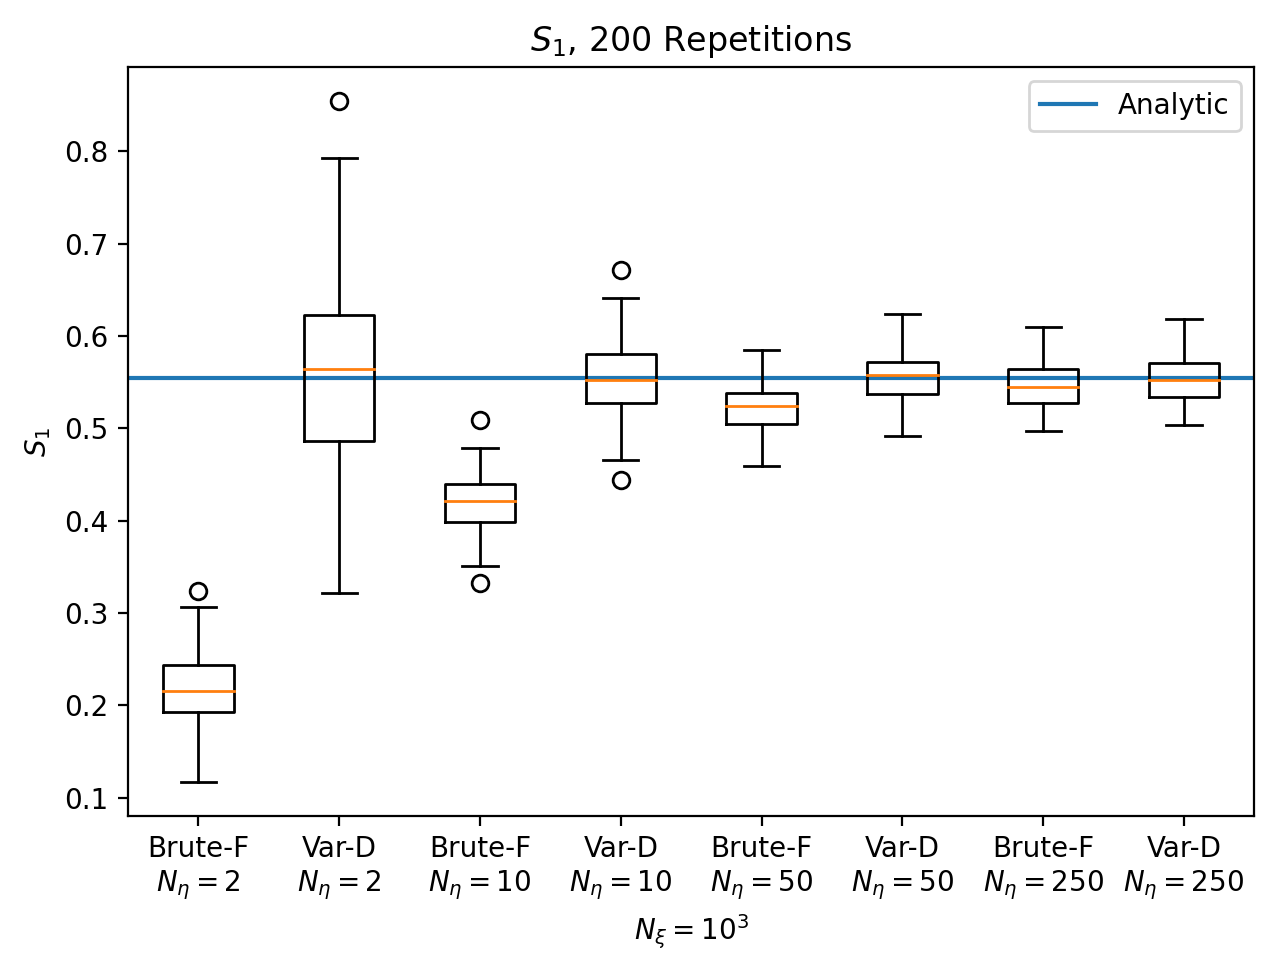
\includegraphics[width=\textwidth]{figures/ishi_s1_boxplot_c5.png}
    \caption{For the Ishigami function with added stochasticity, comparing distributions of $\S{1}$ calculated using a variance deconvolution (Var-D) vs. a standard approach (Brute-F) with the Saltelli estimator. $\Nxi=10^3$ in every case, with $\Neta$ increasing from left to right within a single plot. Analytic indices reported as solid horizontal line.}
    \label{fig:ishigami-s1}
\end{figure} \hfill
\begin{figure}[b]
    \centering
    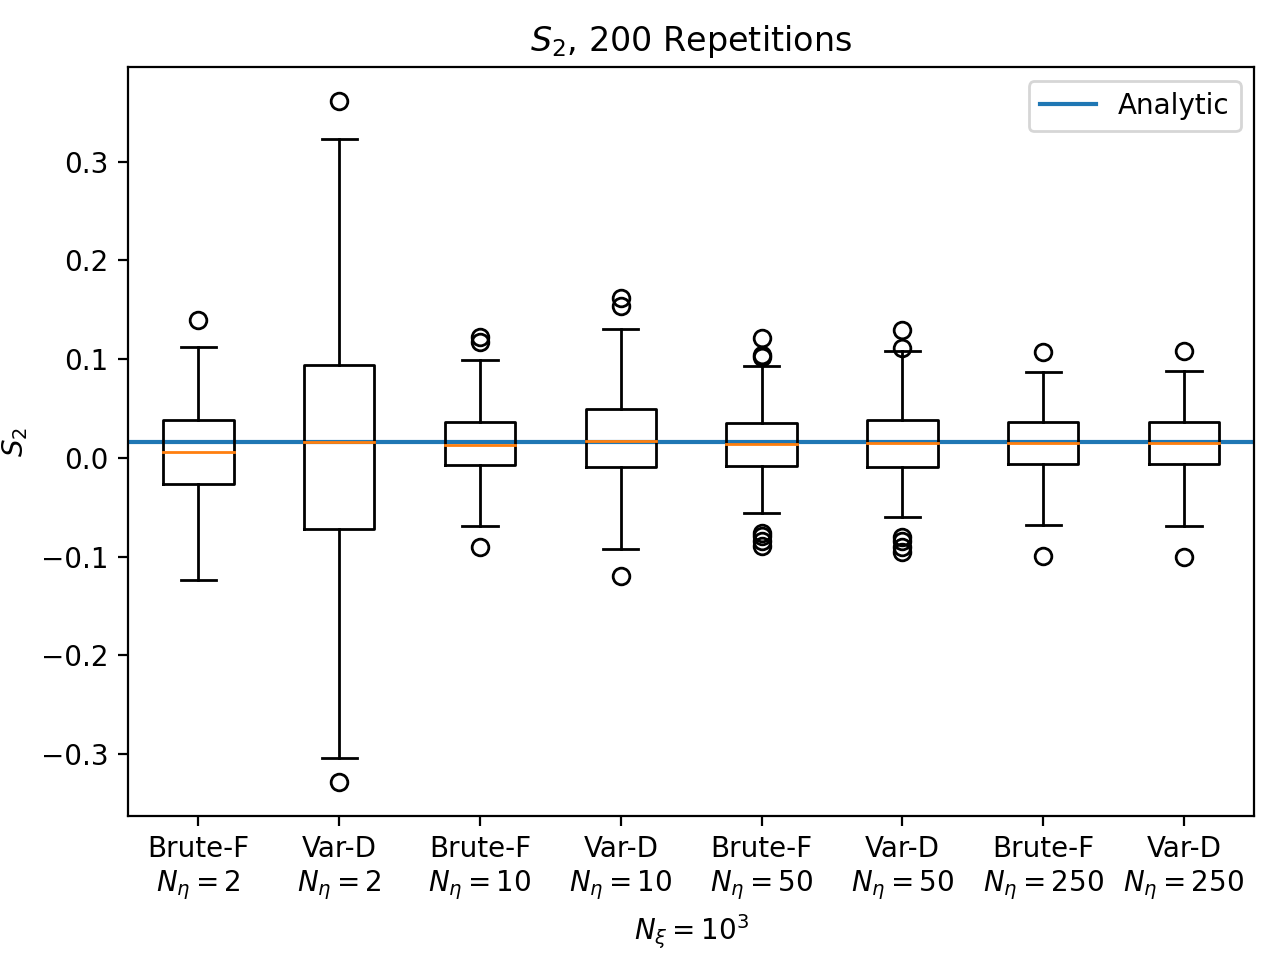
\includegraphics[width=\textwidth]{figures/ishi_s2_boxplot_c5.png}
    \caption{For the Ishigami function with added stochasticity, comparing distributions of $\S{2}$ calculated using a variance deconvolution (Var-D) vs. a standard approach (Brute-F) with the Saltelli estimator. $\Nxi=10^3$ in every case, with $\Neta$ increasing from left to right within a single plot. Analytic indices reported as solid horizontal line.}
    \label{fig:ishigami-s2}
\end{figure}
\begin{figure}[b]
    \centering
    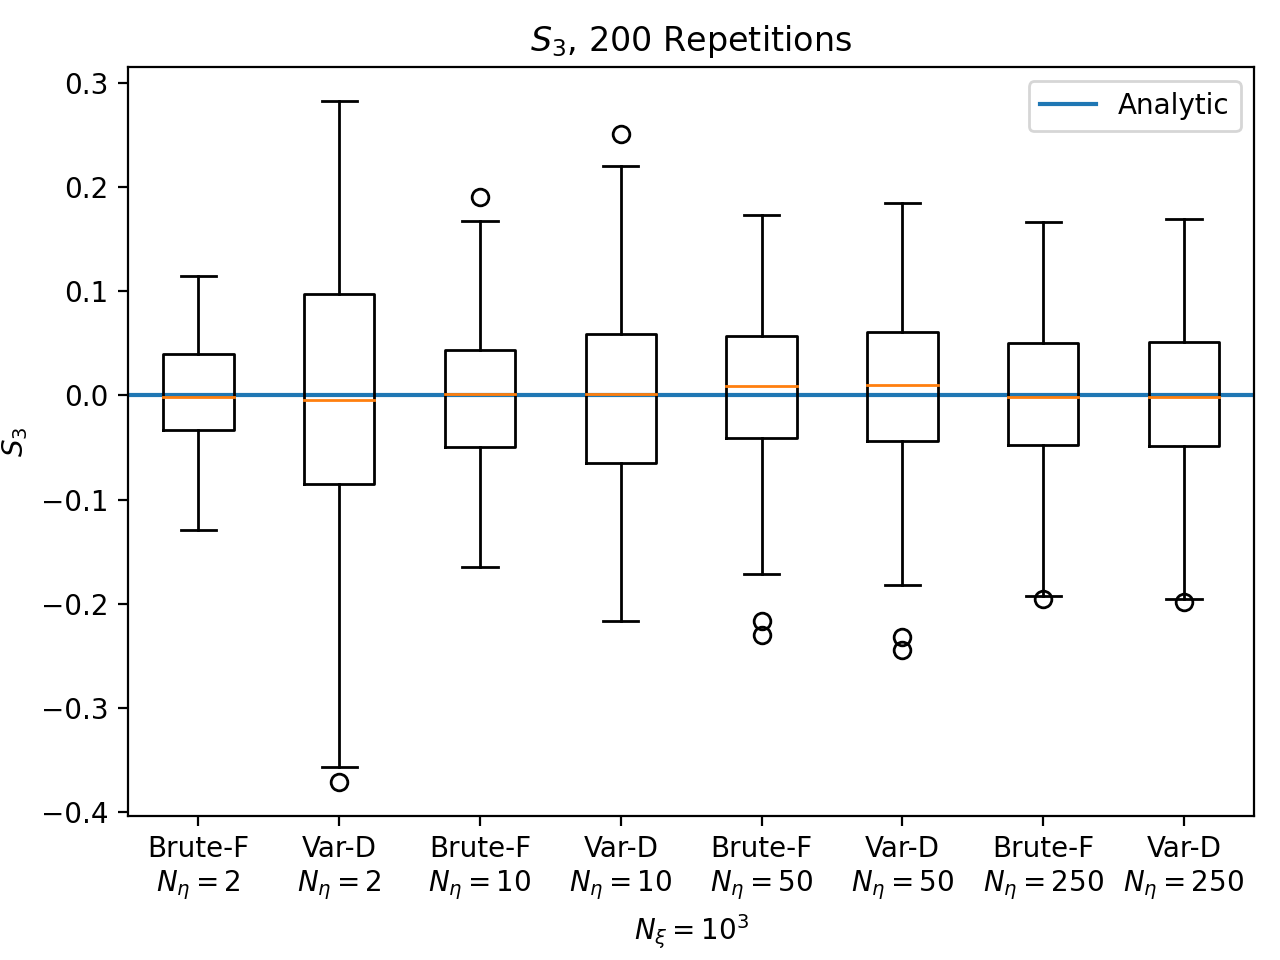
\includegraphics[width=\textwidth]{figures/ishi_s3_boxplot_c5.png}
    \caption{For the Ishigami function with added stochasticity, comparing distributions of $\S{3}$ calculated using a variance deconvolution (Var-D) vs. a standard approach (Brute-F) with the Saltelli estimator. $\Nxi=10^3$ in every case, with $\Neta$ increasing from left to right within a single plot. Analytic indices reported as solid horizontal line.}
    \label{fig:ishigami-s3}
\end{figure}
\begin{figure}[b]
    \centering
    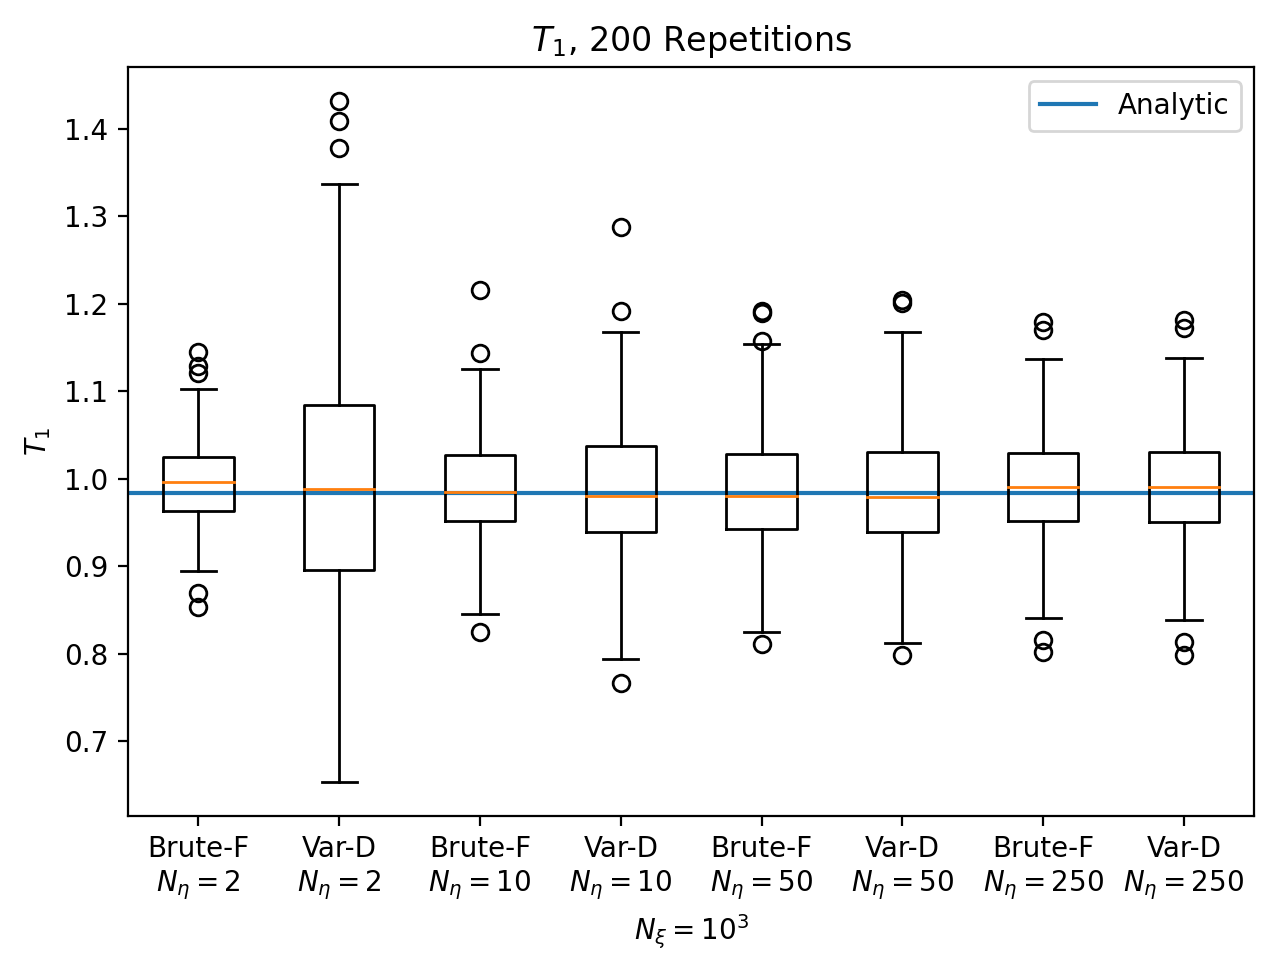
\includegraphics[width=\textwidth]{figures/ishi_t1_boxplot_c5.png}
    \caption{For the Ishigami function with added stochasticity, comparing distributions of $\T{1}$ calculated using a variance deconvolution (Var-D) vs. a standard approach (Brute-F) with the Saltelli estimator. $\Nxi=10^3$ in every case, with $\Neta$ increasing from left to right within a single plot. Analytic indices reported as solid horizontal line.}
    \label{fig:ishigami-t1}
\end{figure}
\begin{figure}[b]
    \centering
    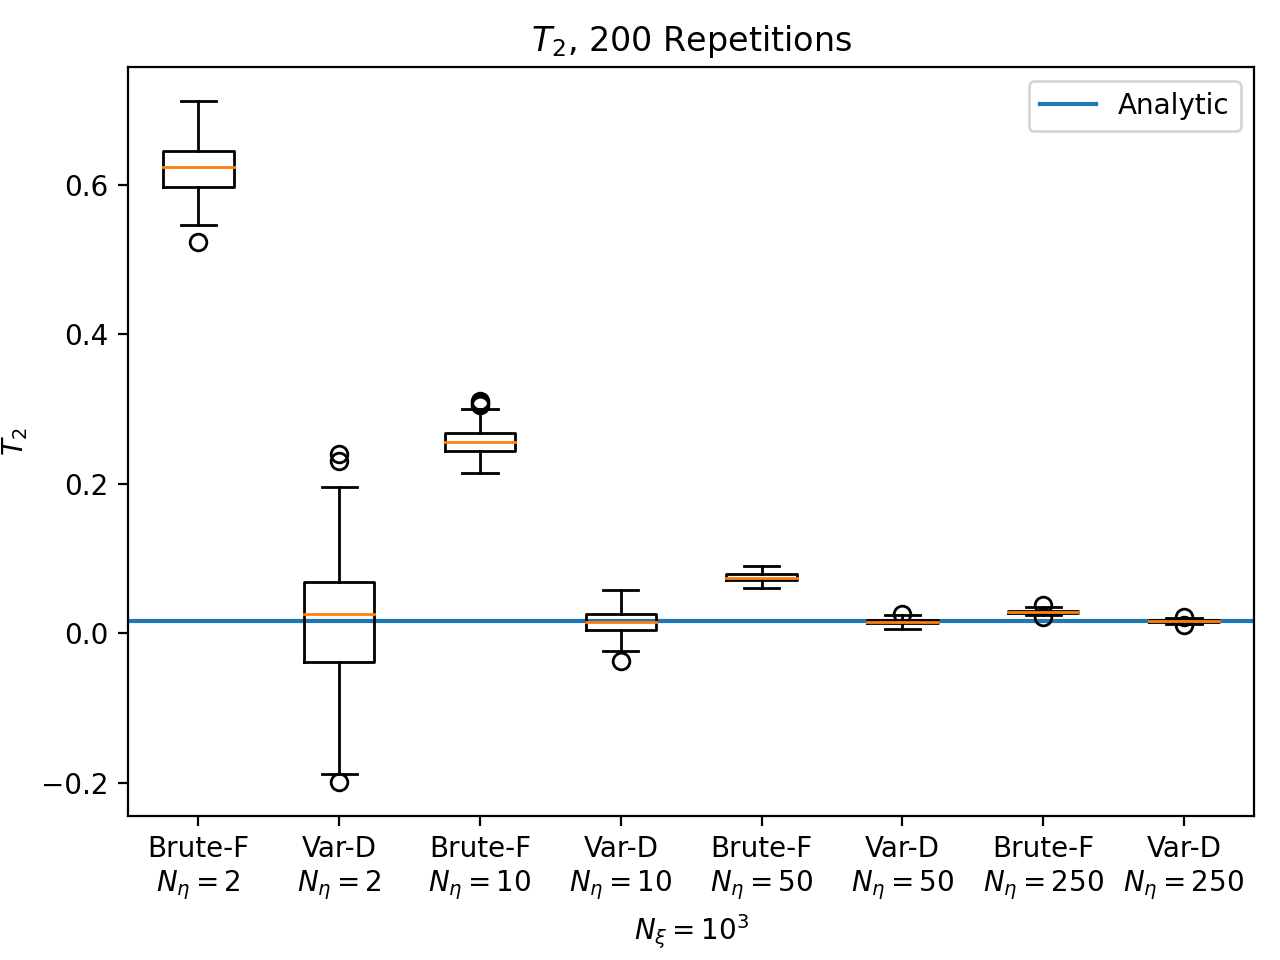
\includegraphics[width=\textwidth]{figures/ishi_t2_boxplot_c5.png}
    \caption{For the Ishigami function with added stochasticity, comparing distributions of $\T{2}$ calculated using a variance deconvolution (Var-D) vs. a standard approach (Brute-F) with the Saltelli estimator. $\Nxi=10^3$ in every case, with $\Neta$ increasing from left to right within a single plot. Analytic indices reported as solid horizontal line.}
    \label{fig:ishigami-t2}
\end{figure}
\begin{figure}[b]
    \centering
    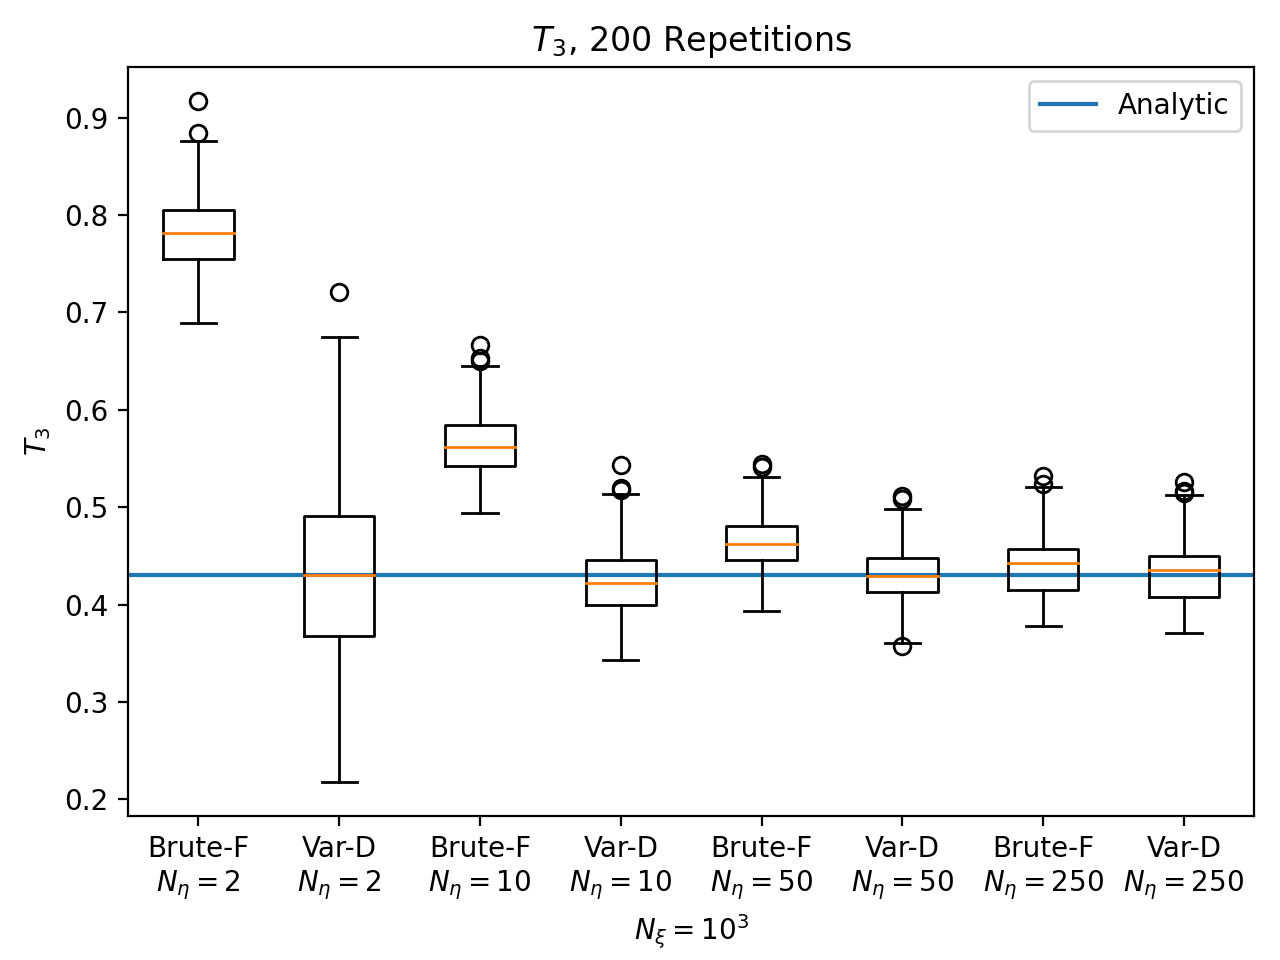
\includegraphics[width=\textwidth]{figures/ishi_t3_boxplot_c5.png}
    \caption{For the Ishigami function with added stochasticity, comparing distributions of $\T{3}$ calculated using a variance deconvolution (Var-D) vs. a standard approach (Brute-F) with the Saltelli estimator. $\Nxi=10^3$ in every case, with $\Neta$ increasing from left to right within a single plot. Analytic indices reported as solid horizontal line.}
    \label{fig:ishigami-t3}
\end{figure}

% \begin{figure}
% 	\centering
%     \begin{subfigure}[b]{0.3\textwidth}
%         \centering
%         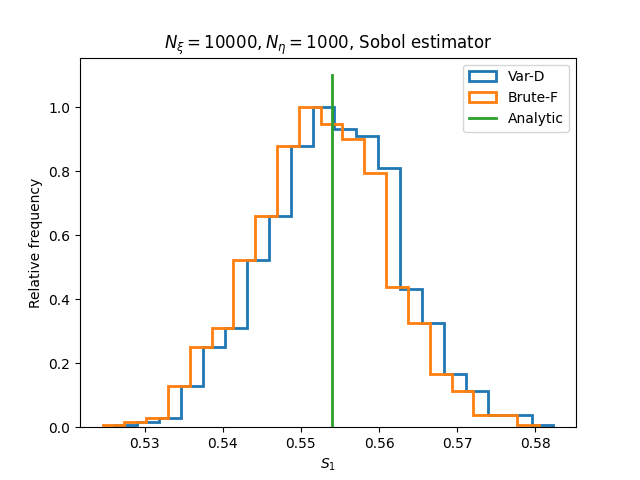
\includegraphics[width=\textwidth]{figures/s1_exp.png}
%         \caption{Computing $\S{1}$ using the Saltelli estimator.}
%         \label{fig:s1}
%     \end{subfigure} \hfill
%     \begin{subfigure}[b]{0.3\textwidth}
%         \centering
%         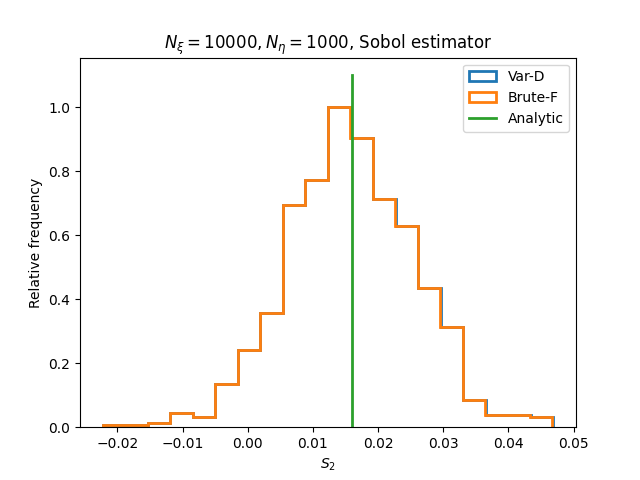
\includegraphics[width=\textwidth]{figures/s2_exp.png}
%         \caption{Computing $\S{2}$ using the Saltelli estimator.}
%         \label{fig:s1}
%     \end{subfigure} \hfill
%     \begin{subfigure}[b]{0.3\textwidth}
%         \centering
%         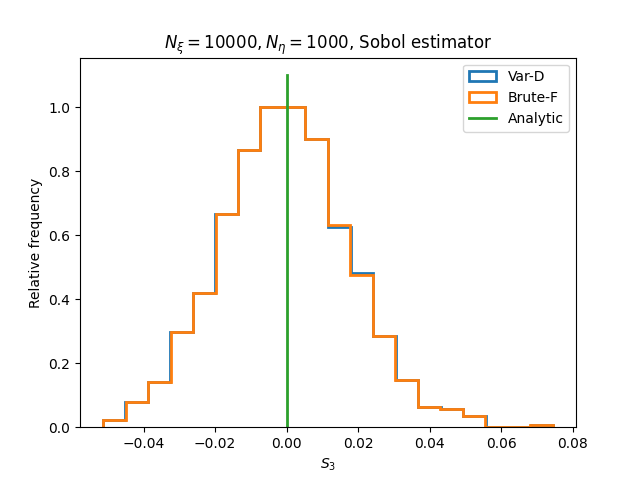
\includegraphics[width=\textwidth]{figures/s3_exp.png}
%         \caption{Computing $\S{3}$ using the Saltelli estimator.}
%         \label{fig:s1}
%     \end{subfigure} \hfill
%     \begin{subfigure}[b]{0.3\textwidth}
%         \centering
%         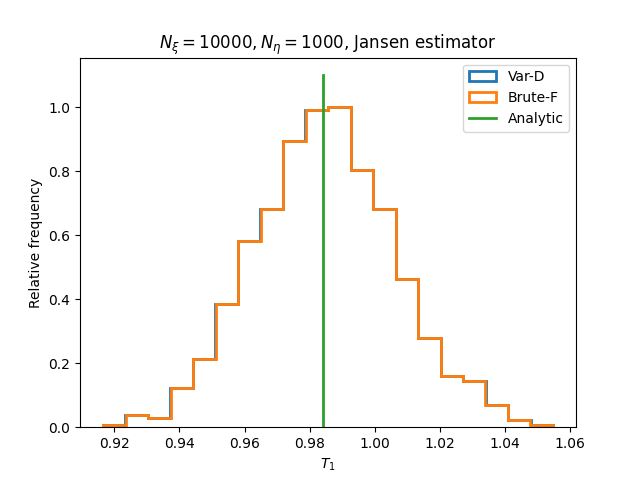
\includegraphics[width=\textwidth]{figures/t1_exp.png}
%         \caption{Computing $\T{1}$ using the Saltelli estimator.}
%         \label{fig:s1}
%     \end{subfigure} \hfill
%     \begin{subfigure}[b]{0.3\textwidth}
%         \centering
%         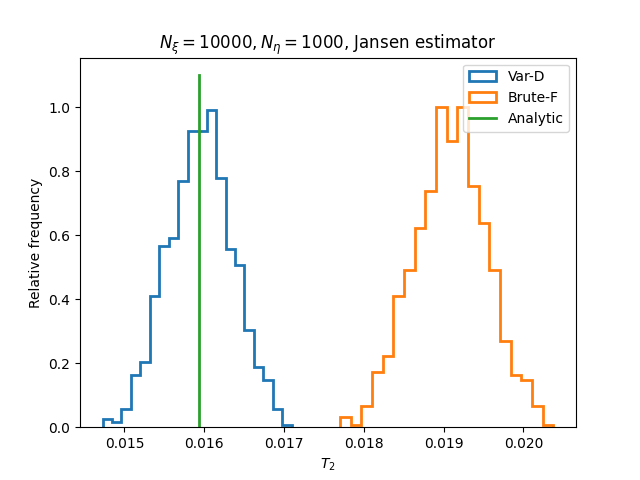
\includegraphics[width=\textwidth]{figures/t2_exp.png}
%         \caption{Computing $\T{2}$ using the Saltelli estimator.}
%         \label{fig:s1}
%     \end{subfigure} \hfill
%     \begin{subfigure}[b]{0.3\textwidth}
%         \centering
%         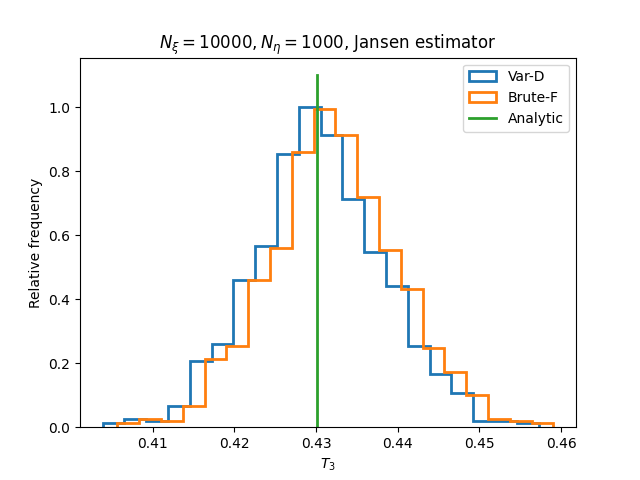
\includegraphics[width=\textwidth]{figures/t3_exp.png}
%         \caption{Computing $\T{3}$ using the Saltelli estimator.}
%         \label{fig:s1}
%     \end{subfigure} \hfill
%     \caption{Comparing the distributions of first- and total-order indices with $\Neta$ increased $200x$ vs Fig.~\ref{fig:ishigami_low}. PDF created with 1\,000 repetitions. Analytic indices reported as solid vertical line.}
% 	\label{fig:ishigami_high}
% \end{figure}

\subsection{Radiation transport test problem}
We next perform GSA on a test neutron transport problem solved using Monte Carlo radiation transport methods~\cite{lux-koblinger-90}. 
The problem is based on the steady-state C5G7 benchmark, a nuclear reactor benchmark developed by the OECD/NEA~\cite{c5g7-2005}. 
We simplify the design by reducing to one dimension in space with three materials: uranium dioxide (UO$_2$) fuel, water moderator, and a control rod. 
There is a constant source, uniform in energy across all groups, at the spatial halfway point.
The neutron energy spectrum is divided into 7 energy groups and we use the cross-sections from the C5G7 benchmark.
Parameter uncertainty is introduced in five independent factors: the densities of 1) the fuel, 2) the moderator, and 3) the control rod were allowed to vary uniformly $\pm 70\%$; 4) the ratio of fuel-width to moderator-width and 5) the control-rod thickness were both allowed to vary uniformly between 0.2 and 0.8. 
We define two quantities of interest as a function of space: the scalar flux of the first two energy groups, $\phi_F (x)$, and the scalar flux of the remaining five energy groups $\phi_S(x)$.

For reference, using $\Nxi=5 \times 10^5$ and $\Neta=10^5$, Figure~\ref{fig:flux} shows $\phi_F (x)$ and $\phi_S (x)$. Figure~\ref{fig:indices} shows the full set of first- and total- order indices for both QoIs.
At such a high $\Neta$, the lines for $\pollSsalt{i}$ and $\pollTsalt{i}$ overlap exactly with those of $\unpollSsalt{i}$ and $\unpollTsalt{i}$, respectively.
The faster group flux $\phi_F$ is most sensitive across space to $\xi_2$, the density of the moderator, which is understandable as the density of the moderator will greatly impact the number of neutrons and their energies everywhere in the problem. 
The control rod's density ($\xi_3$) and thickness ($\xi_5$) are most impactful for the slower group flux, with both having large inflection points at the nominal moderator--control rod boundary at $x=1.5$.
This is understandable as the control rod is a primarily thermal absorber.

\begin{figure}[ht]
    \centering
    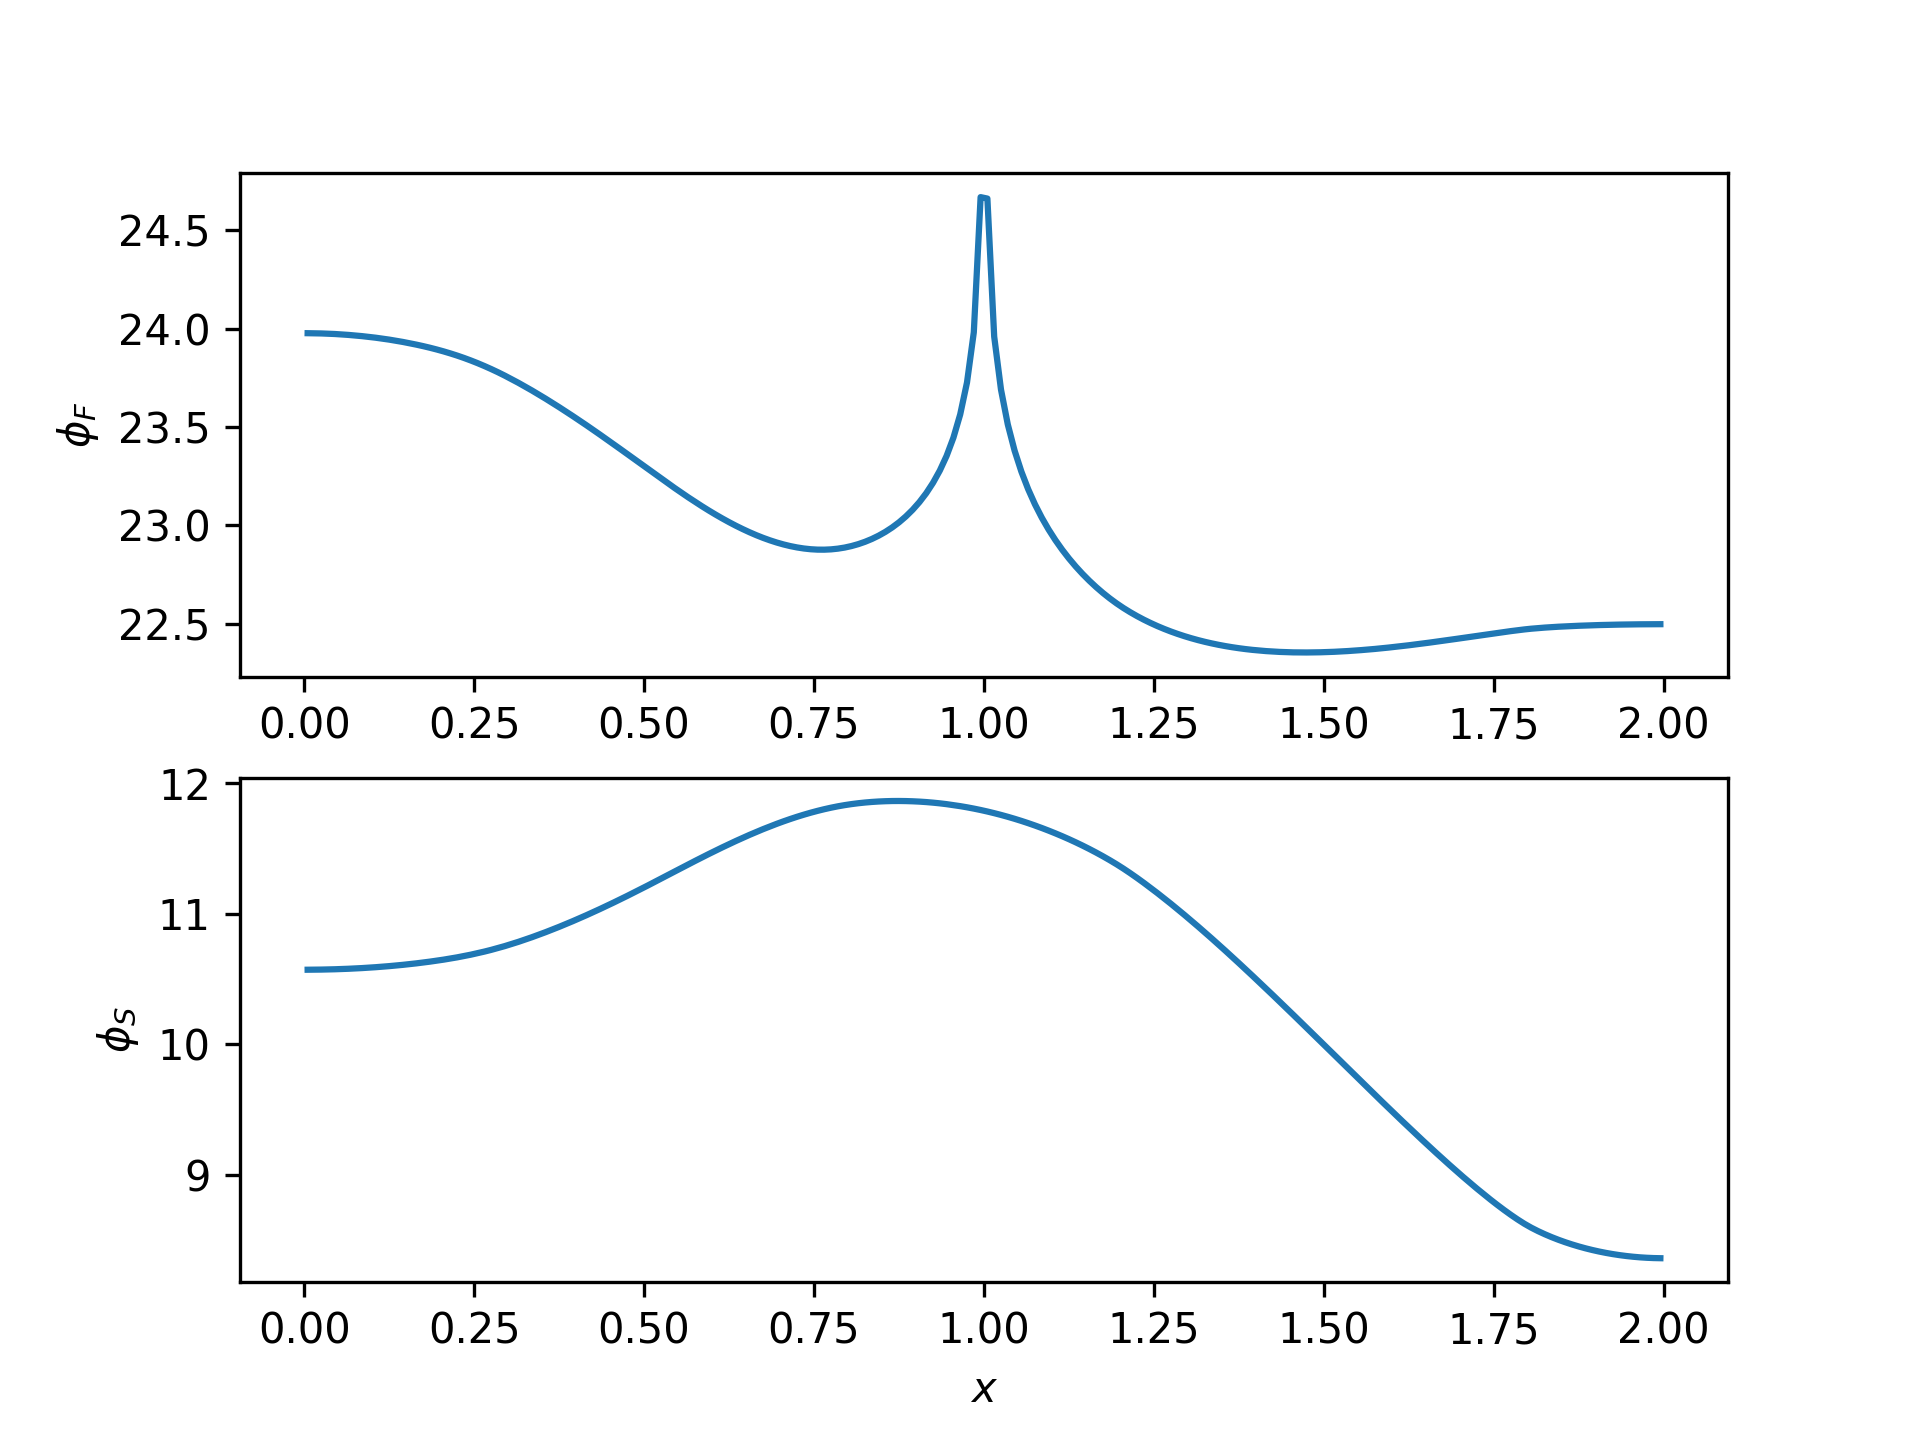
\includegraphics{figures/flux.png} 
    \caption{Average scalar flux with five uncertain parameters using $\Nxi=5 \times 10^5$, $\Neta=10^5$.}
    \label{fig:flux}
\end{figure}

\begin{figure}[ht]
    \centering
    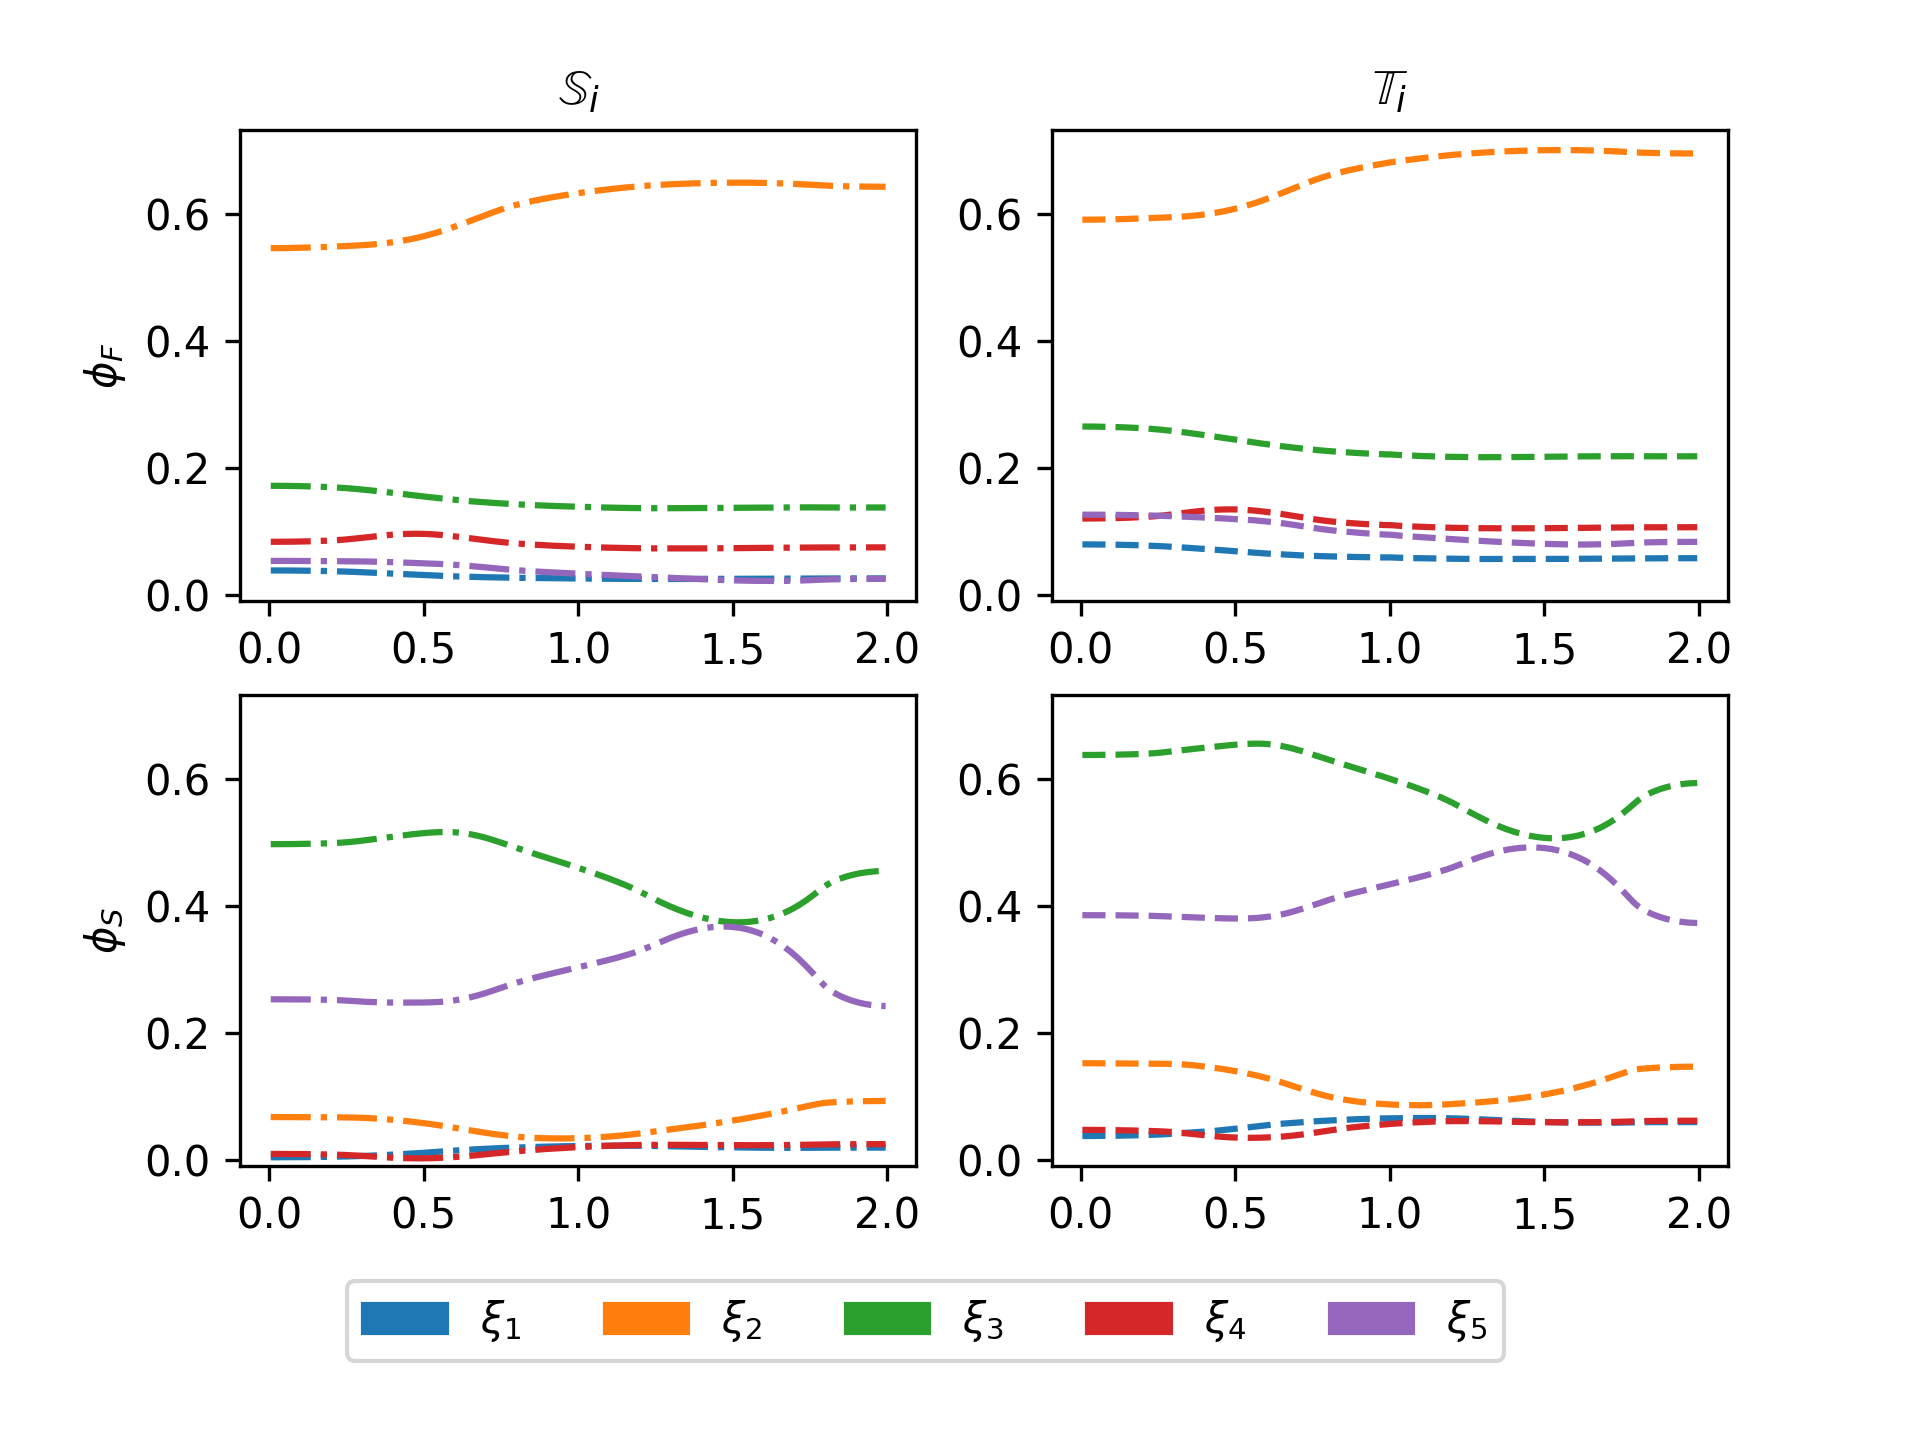
\includegraphics{figures/indices.png}
    \caption{Full set of first- and total- order indices of $\phi_F$ and $\phi_S$ using $\Nxi=5 \times 10^5$, $\Neta=10^5$. Standard and corrected estimators exactly overlap. Uncertain factors: the densities of 1) the fuel, 2) the moderator, 3) and the control rod were allowed to vary uniformly $\pm 70\%$; 4) the ratio of fuel-width to moderator-width and 5) the control-rod thickness were both allowed to vary uniformly between 0.2 and 0.8. }
    \label{fig:indices}
\end{figure}

To see the effect of the variance deconvolution correction, we compare the MSE of the standard and corrected estimators.
In Figure~\ref{fig:mse-fo-fast}, we consider a constant computational cost $\C = \left( \Nxi \times \Neta \right) = 5 \times 10^5$ in two different combinations of $\Nxi$ and $\Neta$.
In the first combination, $\left( \Nxi, \Neta \right) = \left( 5 \times 10^3, 10^2 \right)$, we see that the MSE of the standard estimator is clearly lower than that of the var-d estimator for $\S{1}$ and $\S{5}$. 
Both of these indices are very close to zero (see Figure~\ref{fig:indices}); in this case, the higher variance of the var-d estimator outweighs the bias of the standard estimator.
In the second combination, we have increased $\Nxi$ by a factor of 10 and decreased $\Neta$ by the same factor to keep $\C$ constant.
The variance deconvolution estimator benefits from this configuration, with an MSE that is lower than that of the standard estimator at most locations in $x$. 

This pattern is consistent across QoIs: when indices are close to zero the variance of the variance deconvolution estimator can outweigh the bias of the standard estimator, and for a constant $\C$ the variance deconvolution estimator generally benefits from increasing the $\Nxi$ at the expense of decreasing $\Neta$. 
In Figure~\ref{fig:mse-fo-slow}, we see this for $\S{i} \left[ \phi_S \right]$.
For estimating $\T{i}$, the correction in both the numerator and denominator makes the difference between the standard and variance deconvolution estimators more drastic.
In Figures~\ref{fig:mse-to-fast} and~\ref{fig:mse-to-slow}, we see that the variance deconvolution estimator outperforms the standard across $x$ for both $\phi_F$ and $\phi_S$.

\begin{figure}
    \centering
    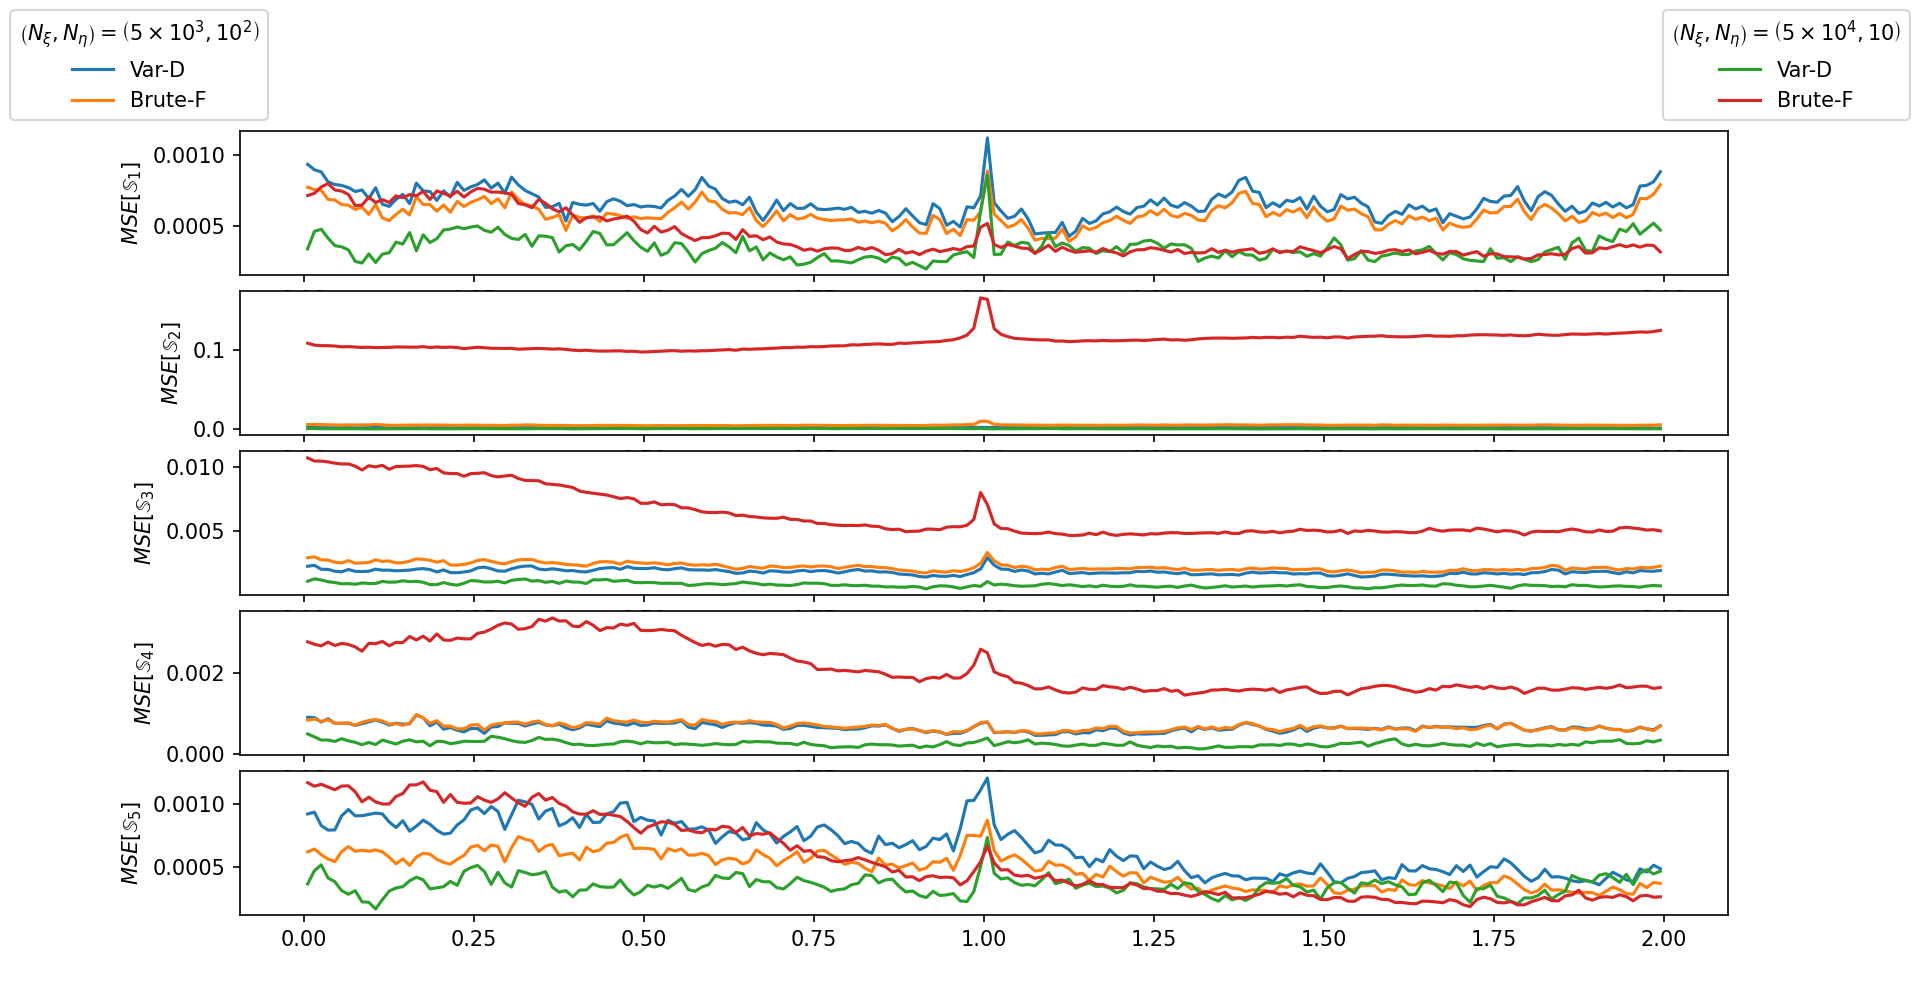
\includegraphics[width=\textwidth]{figures/mse_firstorder_fast.png}
    \caption{$MSE\left[\S{i}\right]$ for $\phi_F$, constant computational cost $\C = \left( \Nxi \times \Neta \right) = 5 \times 10^5$.}
    \label{fig:mse-fo-fast}
\end{figure}

\begin{figure}
    \centering
    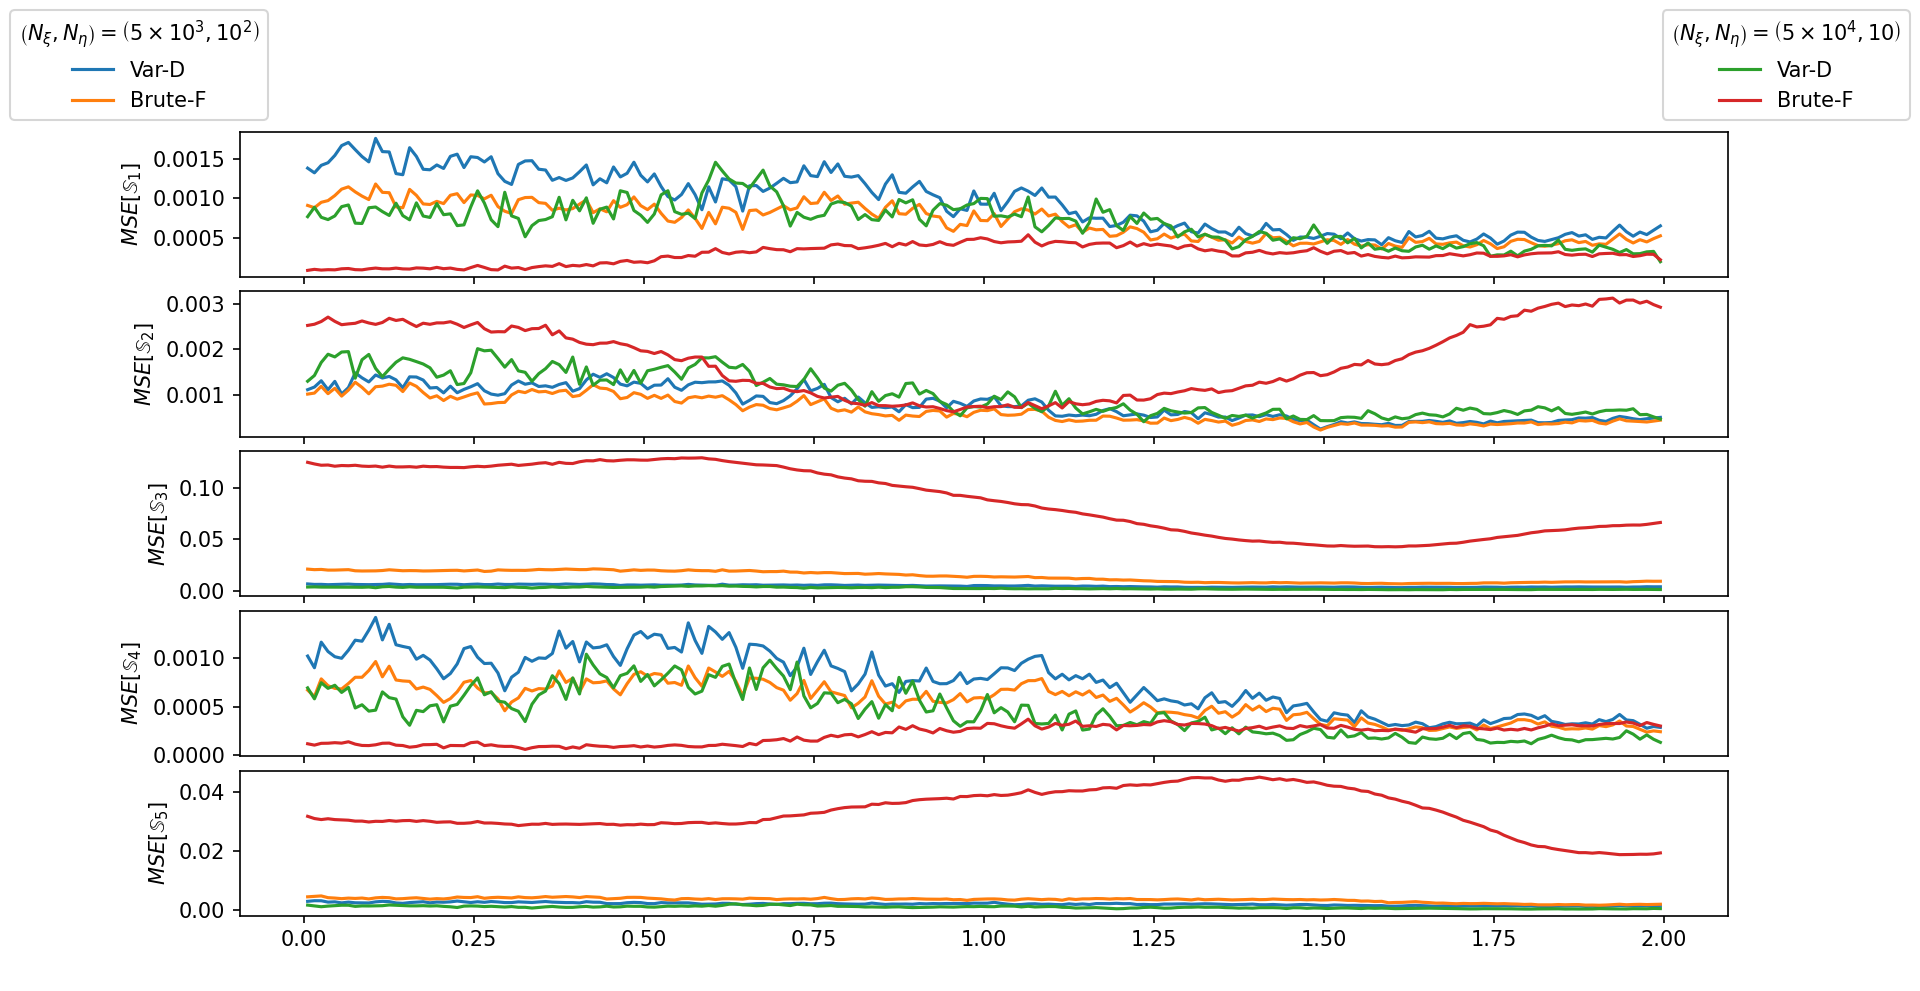
\includegraphics[width=\textwidth]{figures/mse_firstorder_slow.png}
    \caption{$MSE\left[\S{i}\right]$ for $\phi_S$, constant computational cost $\C = \left( \Nxi \times \Neta \right) = 5 \times 10^5$.}
    \label{fig:mse-fo-slow}
\end{figure}

\begin{figure}
    \centering
    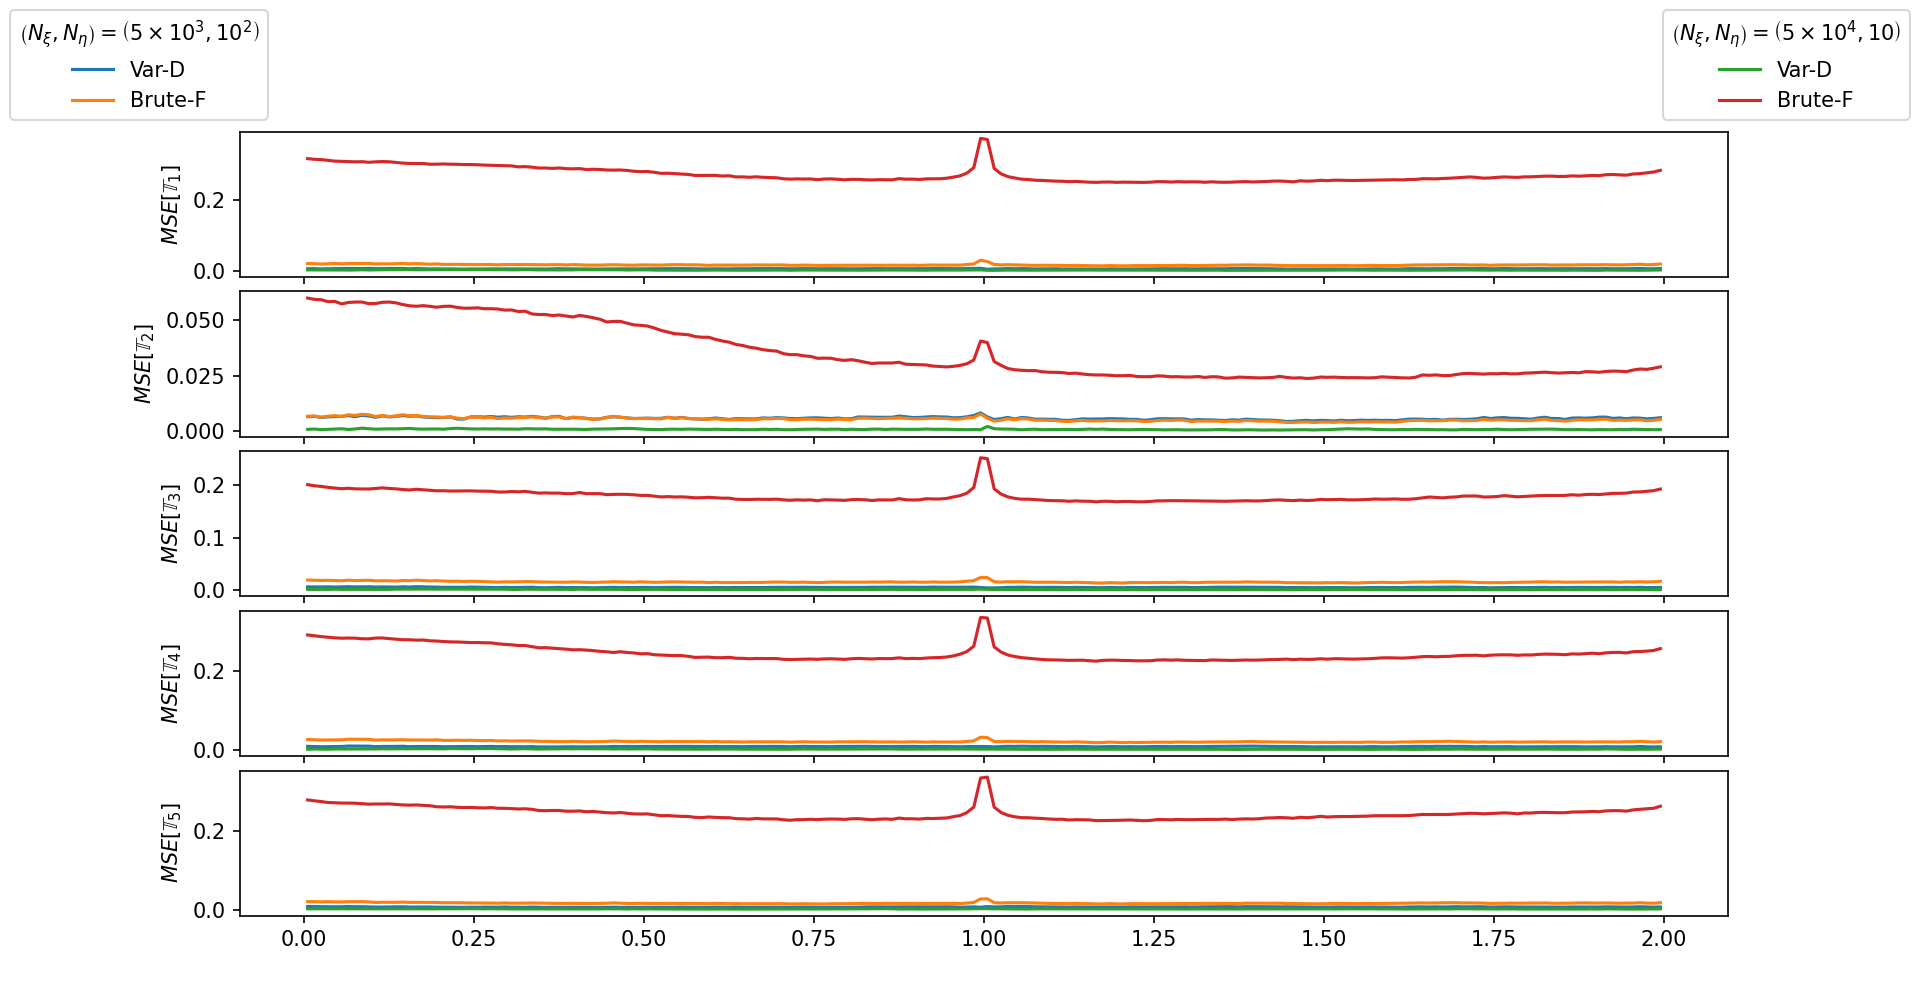
\includegraphics[width=\textwidth]{figures/mse_totalorder_fast.png}
    \caption{$MSE\left[\T{i}\right]$ for $\phi_F$, constant computational cost $\C = \left( \Nxi \times \Neta \right) = 5 \times 10^5$.}
    \label{fig:mse-to-fast}
\end{figure}

\begin{figure}
    \centering
    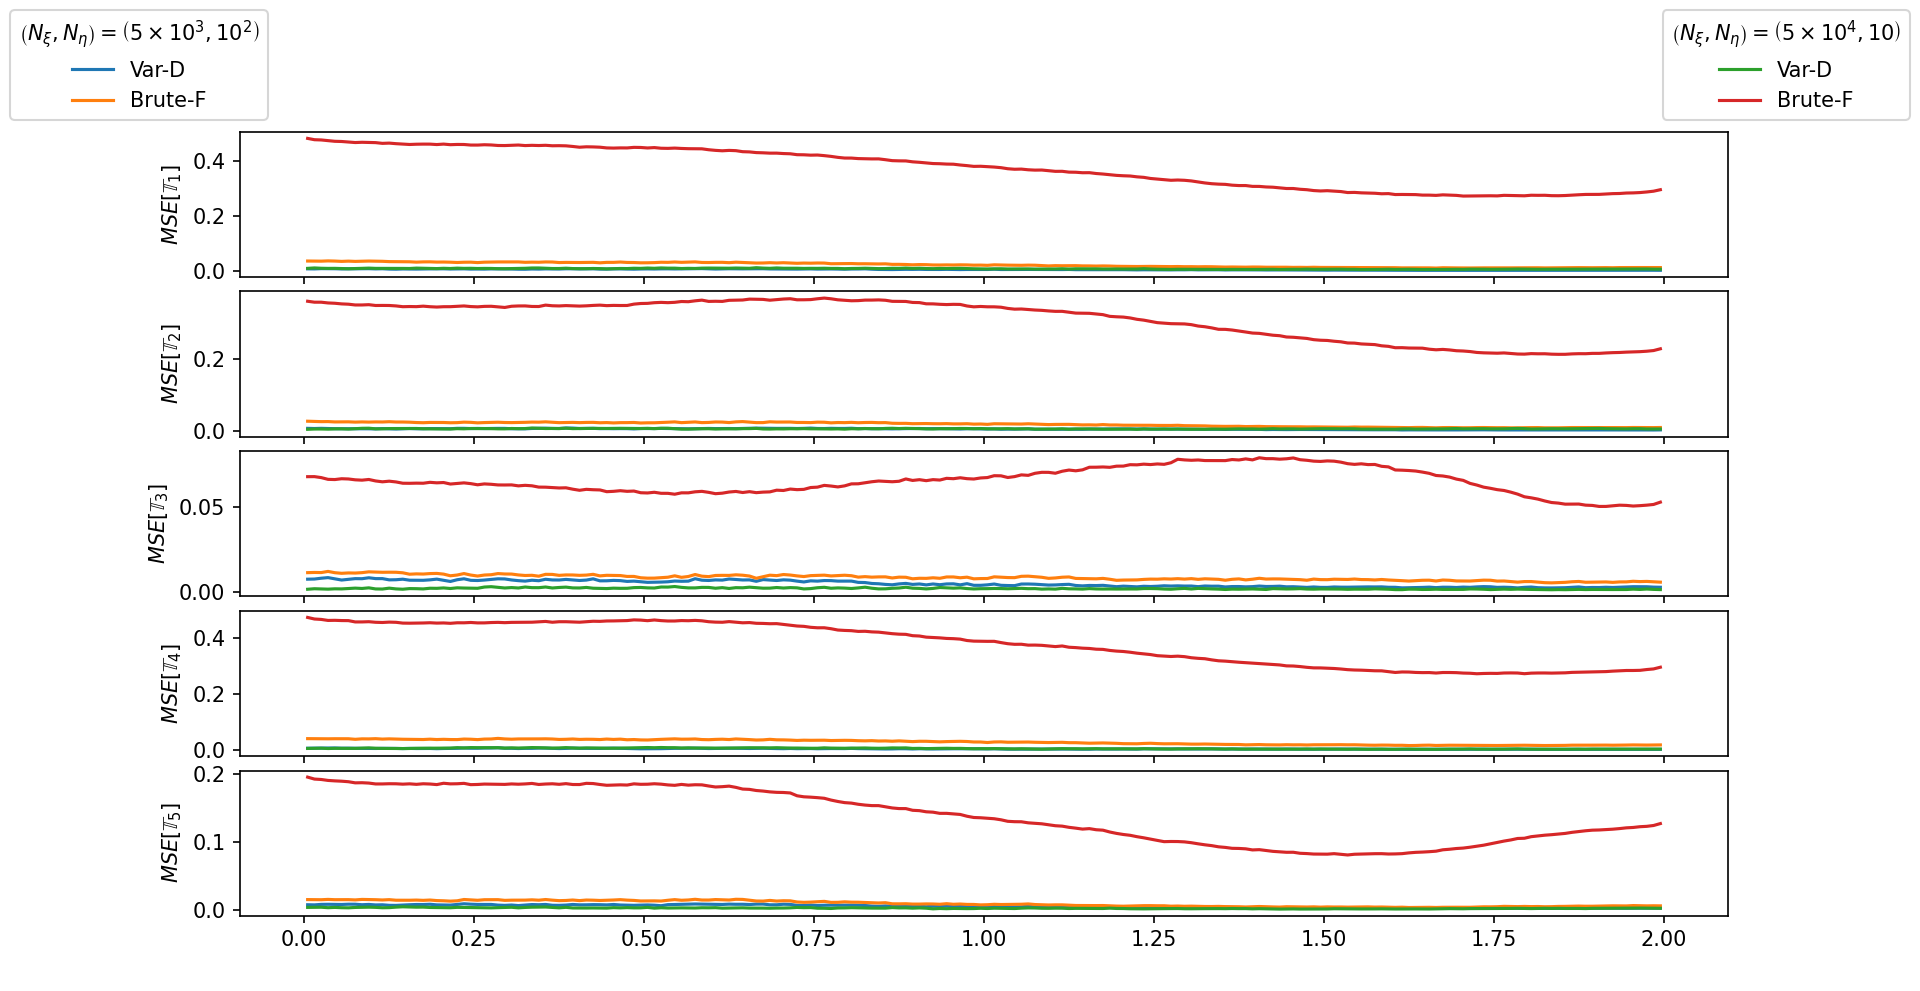
\includegraphics[width=\textwidth]{figures/mse_totalorder_slow.png}
    \caption{$MSE\left[\T{i}\right]$ for $\phi_S$, constant computational cost $\C = \left( \Nxi \times \Neta \right) = 5 \times 10^5$.}
    \label{fig:mse-to-slow}
\end{figure}

We have shown, in this example and the analytic test case, that when increasing computational cost for more accurate estimates of $\S{i}$ and $\T{i}$, putting those computational resources towards increasing $\Nxi$ with the variance deconvolution estimator will improve the accuracy of indices that are not near zero.


\section{Conclusion}
\label{sec:conclusion}
In this paper, we extend the variance deconvolution framework introduced in~\cite{clements-etal-2024} for UQ to global sensitivity analysis (GSA).
Sobol' indices are well-suited and widely used for GSA, and there has been abundant work over the past few decades on the most efficient sampling schemes and estimators for SIs. 
In this work, we analyze the effect on SIs when the underlying solver is stochastic, i.e., has some underlying inherent variability (e.g., Monte Carlo radiation transport solvers).
We build on a previously-developed variance deconvolution estimator which, rather than computing parametric variance by over-resolving the stochastic solver, explicitly quantifies and removes the solver variance from the total observed variance.
We show in closed-form that in general, a stochastic solver will introduce a bias to under-estimate the parametric first-order SIs and over-estimate the parametric total-order SIs. 
We find that though the variance deconvolution version of existing SI estimators can have a higher variance than its standard counterpart, the variance deconvolution version is able to accurately compute the indices for a reduced cost.
When the solver noise contribution was approximately equal to the parameter noise, the variance deconvolution estimator saved 50X computational cost compared to the standard.
When the solver noise was approximately double the parameter noise, the variance deconvolution estimator saved a 250X computational cost.





\section{Mean-squared error from asymptotic limits}
\label{appx:mse}
The law of large numbers and central limit theorem ensure that the estimators $\unpollSsalt{i}$ and $\unpollTsalt{i}$ converge to $\S{i}$ and $\T{i}$ almost surely, i.e., $\lim_{\Nxi \rightarrow \infty} \unpollSsalt{i} = \S{i}$ and $\lim_{\Nxi \rightarrow \infty} \unpollTsalt{i} = \T{i}$.

The estimators $\pollSsalt{i}$ and $\pollTsalt{i}$ converge almost surely to $\Spoll{i}$ and $\Tpoll{i}$ in the limit $\Nxi \rightarrow \infty$, and to $\S{i}$ and $\T{i}$ in the stricter limit $\left( \Nxi, \Neta\right) \rightarrow \infty$.

We assume that the sample estimator $\unpollSsalt{i}$ uses sample sizes $\Nxi$ and $\Neta$ for the sensitivity sampling and stochastic solver samples per realization, respectively.
In the following, we follow the steps of Janon et al. (2014)~\cite{janon-etal-2014} and Azzini et al. (2021)~\cite{azzini-etal-2021} to establish that the asymptotic normality of this estimator is,
\begin{equation}
    \lim_{\Nxi \rightarrow \infty} \sqrt{\Nxi} \left( \unpollSsalt{i} - \S{i} \right) \sim \mathcal{N} \Biggl( 0, \Var{\alpha - \S{i} (\beta - \gamma )} \Biggr) .
\end{equation}

\subsection{Proof: First-order Estimators} \label{sec:proof-first-order}
We define random vector $X$ with mean $\mu_X$, variance $\Sigma_X$, and sample mean $\xavg = \Nxi^{-1} \sumv X_v$, where the statistics of the samples $X_v$ do not depend on $v$:
\begin{align} \label{m4eq:xmatrix}
    X &= \begin{bmatrix} \Qpoll(\bm{B}) \left[ \Qpoll(\bm{A_B^{(i)}}) - \Qpoll(\bm{A}) \right] \\
                        \frac{1}{2} \left( \Qpoll(\bm{A}) - \Qpoll(\bm{B}) \right)^2 \\
                        \frac{1}{2\Neta} \left( \hatSigsqeta(A) + \hatSigsqeta(B) \right)
        \end{bmatrix}
        = \begin{bmatrix} \alpha \\ \beta \\ \gamma \end{bmatrix}, \\
    \mu_X &= \begin{bmatrix} \VE{Q\mid\xi_i} \\ \Var{\Qpoll} \\ \EE{\Sigsqeta}/\Neta \end{bmatrix} 
        = \begin{bmatrix} \mu_\alpha \\ \mu_\beta \\ \mu_\gamma \end{bmatrix}, \\
    \Sigma_X &= \begin{bmatrix}
        \Var{\alpha} & \Cov{\alpha}{\beta} & \Cov{\alpha}{\gamma} \\ 
        \Cov{\alpha}{\beta} & \Var{\beta} & \Cov{\beta}{\gamma} \\
        \Cov{\alpha}{\gamma} & \Cov{\beta}{\gamma} & \Var{\gamma}
    \end{bmatrix} , \\
    X_v &= \begin{bmatrix} \Qpoll(\bm{B})_v \left[ \Qpoll(\bm{A_B^{(i)}})_v - \Qpoll(\bm{A})_v \right] \\
                        \frac{1}{2} \left( \Qpoll(\bm{A})_v - \Qpoll(\bm{B})_v \right)^2 \\
                        \frac{1}{2\Neta} \left( \hatSigsqeta(A)_v + \hatSigsqeta(B)_v \right)
        \end{bmatrix} \iid F(X) .
\end{align}

From the central limit theorem (CLT), we have $\sqrt{\Nxi} \left( \xavg - \mu_X \right) \cond \mathcal{N}_k \left(0, \Sigma_X \right)$. 

\noindent
We define a function $g(a,b,c)$ and its gradient $\nabla g$,
\begin{equation}
    g (a,b,c) = \frac{a}{b - c} , \qquad
    \nabla g (a,b,c) = \left[ \frac{1}{b-c}, \, \frac{-a}{(b-c)^2}, \, \frac{a}{(b-c)^2} \right] ,
\end{equation}
such that we can write 
\begin{gather}
    g \left( \mu_X \right) = \frac{\VE{Q\mid\xi_i}}{\Var{\Qpoll} - \frac{1}{\Neta}\EExi{\Sigsqeta}} = \frac{\VE{Q\mid\xii}}{\Vxi{Q}} = \S{i} ,\\
    g \left( \xavg \right) = \unpollSsalt{i} .
\end{gather}
From the so-called Delta method~\cite{vandervaart-2000}, given function $g$ with gradient $\nabla g$ such that $\nabla g (\mu_X) \defin \nabla_{\mu_X} \neq 0$, 
\begin{equation*}
    \sqrt{\Nxi} \left( g(\xavg) - g(\mu_X) \right) \cond \mathcal{N} \left( 0, \nabla_{\mu_X} \, \Sigma_X \, \nabla_{\mu_X}^T \right) .
\end{equation*}
%
Therefore, we find that the estimator $\unpollSsalt{i}$ is unbiased regardless of stochastic solver sampling size $\Neta$, with variance that depends on both $\Nxi$ and $\Neta$,
\begin{equation}
    \Var{\unpollSsalt{i}} = \frac{\Var{\alpha - \S{i} \left( \beta - \gamma \right)}}{\Vxisq{Q}} .
\end{equation}
Plugging in $\alpha$, $\beta$, and $\gamma$ defined in Eq.~\eqref{m4eq:xmatrix} leads to the result in Eq.~\ref{m4eq:var-s-vd}.

Analysis of standard estimator $\pollSsalt{i}$ follows by defining vector $Y = \left[ \alpha, \beta, 0 \right]^T$ such that $g(\mu_Y) = \Spoll{i}$ and $g(\yavg) = \pollSsalt{i}$. 
Then,
\begin{equation*}
    \sqrt{\Nxi} \left( g(\yavg) - g(\mu_Y) \right) \cond \mathcal{N} \left( 0, \nabla_{\mu_Y} \, \Sigma_X \, \nabla_{\mu_Y}^T \right) .
\end{equation*}
%
Therefore, we find that $\pollSsalt{i}$ is a biased estimator of $\S{i}$, where the magnitude of the bias depends on $\Neta$, with variance that depends on both $\Nxi$ and $\Neta$,
\begin{align}
    \bias{\pollSsalt{i}, \S{i}} &= \left( \EE{\pollSsalt{i}} - \S{i} \right)^2 \\
    &= \left( \Spoll{i} - \S{i} \right)^2 \\
    &= \S{i}^2 \left( \frac{\Vxi{Q}}{\Var{\Qpoll}} - 1 \right)^2 \\
    &= \frac{\S{i}^2}{\Neta^2} \frac{\EExisq{\Sigsqeta}}{\Vsq{\Qpoll}}
\end{align}
\begin{align}
        \Var{\pollSsalt{i}} &= \frac{\Var{\alpha - \Spoll{i}\beta}}{\Vsq{\Qpoll}} \\
        &= \frac{1}{\Vsq{\Qpoll}}\Var{\alpha} + \frac{\Vxisq{Q}}{\Var{\Qpoll}^4}\S{i}^2 \Var{\beta} - 2 \frac{\Vxi{Q}}{\Var{\Qpoll^3}} \S{i} \Cov{\alpha}{\beta}
\end{align}
Plugging in $\alpha$ and $\beta$ defined in Eq.~\eqref{m4eq:xmatrix} leads to the result in Eq.~\ref{m4eq:var-s-stan}.

%
%
%
%
\subsection{Proof: Total-order Estimators}
To analyze $\unpollTsalt{i}$ and $\pollTsalt{i}$, we follow the same process as for the first-order estimators above.
We define random vector $X$ with mean $\mu_X$, variance $\Sigma_X$, and sample mean $\xavg = \Nxi^{-1} \sumv X_v$, where the statistics of the samples $X_v$ do not depend on $v$:
\begin{align} \label{m4eq:t-xmatrix}
    X &= \begin{bmatrix} \frac{1}{2} \left( \Qpoll(\bm{B_A^{(i)}}) - \Qpoll(\bm{B}) \right)^2 \\
                        \frac{1}{2} \left( \Qpoll(\bm{A}) - \Qpoll(\bm{B}) \right)^2 \\
                        \frac{1}{2\Neta} \left( \hatSigsqeta(\bm{A}) + \hatSigsqeta(\bm{B}) \right) \\
                        \frac{1}{2\Neta} \left( \hatSigsqeta(\bm{B_A^i}) + \hatSigsqeta(\bm{B}) \right)
        \end{bmatrix}
        = \begin{bmatrix} \alpha \\ \beta \\ \gamma \\ \delta \end{bmatrix}, \\
    \mu_X &= \begin{bmatrix} \VE{Q\mid\xi_i} \\ \Var{\Qpoll} \\ \EE{\Sigsqeta}/\Neta \\ \EE{\Sigsqeta}/\Neta \end{bmatrix} 
        = \begin{bmatrix} \mu_\alpha \\ \mu_\beta \\ \mu_\gamma \\ \mu_\delta \end{bmatrix}, \\
    \Sigma_X &= \begin{bmatrix}
        \Var{\alpha} & \Cov{\alpha}{\beta} & \Cov{\alpha}{\gamma} & \Cov{\alpha}{\delta} \\ 
        \Cov{\alpha}{\beta} & \Var{\beta} & \Cov{\beta}{\gamma} & \Cov{\beta}{\delta} \\
        \Cov{\alpha}{\gamma} & \Cov{\beta}{\gamma} & \Var{\gamma} & \Cov{\gamma}{\delta} \\
        \Cov{\alpha}{\delta} & \Cov{\beta}{\delta} & \Cov{\gamma}{\delta} & \Var{\delta}
    \end{bmatrix} .
\end{align}
We define a function $g(a,b,c,d)$ and its gradient $\nabla g$,
\begin{align}
    g (a,b,c,d) &= \frac{a-d}{b - c} \\
    \nabla g (a,b,c,d) &= \left[ \frac{1}{b-c}, \, \frac{-(a-d)}{(b-c)^2}, \, \frac{(a-d)}{(b-c)^2}, \, \frac{-1}{b-c} \right] ,
\end{align}
such that we can write $g(\mu_X) = \T{i}$ and $g(\xavg) = \unpollTsalt{i}$.
%
Therefore, we find that the estimator $\unpollTsalt{i}$ is unbiased regardless of stochastic solver sampling size $\Neta$, with variance that depends on both $\Nxi$ and $\Neta$,
\begin{equation}
    \Var{\unpollTsalt{i}} = \frac{\Var{\alpha - \delta - \T{i} \left( \beta - \gamma \right)}}{\Vxisq{Q}} .
\end{equation}
Plugging in $\alpha$, $\beta$, $\gamma$, and $\delta$ defined in Eq.~\eqref{m4eq:t-xmatrix} leads to the result in Eq.~\ref{m4eq:var-t-vd}.

Analysis of standard estimator $\pollTsalt{i}$ follows by defining vector $Y = \left[ \alpha, \beta, 0, 0 \right]^T$ such that $g(\mu_Y) = \Tpoll{i}$ and $g(\yavg) = \pollTsalt{i}$. 
%
Therefore, we find that $\pollTsalt{i}$ is a biased estimator of $\T{i}$, where the magnitude of the bias depends on $\Neta$, with variance that depends on both $\Nxi$ and $\Neta$,
\begin{align}
    \bias{\pollTsalt{i}, \T{i}} &= \left( \EE{\pollTsalt{i}} - \T{i} \right)^2 \\
    &= \left( \Tpoll{i} - \T{i} \right)^2 \\
    &= \T{i}^2 \left( \frac{\Vxi{Q}\pollE{\ni}}{\Var{\Qpoll}\E{\ni}} - 1 \right)^2 \\
    &= \frac{\T{i}^2}{\Neta^2} \frac{\EExisq{\Sigsqeta} \V{\ni}^2}{\Vsq{\Qpoll} \E{\ni}^2} ,
\end{align}
\begin{align}
        \Var{\pollTsalt{i}} &= \frac{\Var{\alpha - \Tpoll{i}\beta}}{\Vsq{\Qpoll}} \\
        &= \frac{1}{\Vsq{\Qpoll}}\Var{\alpha} + \frac{\Vxisq{Q} \pollE{\ni}^2 }{\Var{\Qpoll}^4 \E{\ni}^2}\T{i}^2 \Var{\beta} - 2 \frac{\Vxi{Q} \pollE{\ni}}{\Var{\Qpoll^3}\E{\ni}} \T{i} \Cov{\alpha}{\beta} .
\end{align}
Plugging in $\alpha$ and $\beta$ defined in Eq.~\eqref{m4eq:t-xmatrix} leads to the result in Eq.~\ref{m4eq:var-t-stan}.





\bibliographystyle{elsarticle-num}
\bibliography{biblio}


\end{document}
\endinput

